\documentclass[preprint,12pt]{elsarticle}

\usepackage{amsmath,amssymb}
\usepackage{graphicx}
\usepackage{booktabs}
\usepackage{multirow}
\usepackage{siunitx}
\usepackage{float}
\usepackage{hyperref}
\usepackage{tikz}
\usetikzlibrary{positioning,arrows.meta,fit,backgrounds,shapes.geometric}
\usepackage{todonotes}

\journal{Medical Image Analysis}

\begin{document}

\begin{frontmatter}

  \title{Architecture-Agnostic Self-Supervised Diffusion MRI Denoising with Hybrid Random Gradient Subsets}

  \author[inst1]{Francisco Hernandez-Sepulveda}
  \ead{jose.sepulveda@cimat.mx}

  \author[inst1]{Mariano Rivera\corref{cor1}}
  \ead{mrivera@cimat.mx}
  \cortext[cor1]{Corresponding author.}

  \address[inst1]{Centro de Investigacion en Matematicas, Guanajuato, Mexico}

  \begin{abstract}
    Diffusion-weighted magnetic resonance imaging (DW-MRI) provides clinically and scientifically valuable measures of brain tissue microstructure, but its reliability is limited by low signal-to-noise ratio, acquisition-dependent noise, and the cost of repeated measurements. Self-supervised denoising is therefore attractive because clean reference images are rarely available. This study evaluates Hybrid Random Gradient Subset (Hybrid RGS), an architecture-agnostic framework designed to preserve denoising performance with limited angular context by combining non-target diffusion information with voxel-wise masking of the target volume. Each training and inference sample contains one masked target and only $K-1$ randomly sampled non-target gradients, with $K\ll G$, rather than conditioning simultaneously on many or all available directions. This reduced per-sample gradient requirement limits input dimensionality while exposing the model to diverse angular contexts across iterations. We instantiate Hybrid RGS with recurrent-convolutional, transformer-style, and independent lightweight two-dimensional backbones to assess whether the same sampling-and-masking objective transfers across architectures rather than to identify a single superior model. On D-Brain data corrupted with synthetic Rician noise, Hybrid RGS substantially improves upon Patch2Self and MD-S2S in image-domain region-of-interest (ROI) metrics, whereas MP-PCA remains a strong baseline for fractional anisotropy (FA) preservation. Ablations show that random gradient sampling outperforms sequential windows in ROI PSNR. A fixed cross-model setting of $K=16$ favors DRCNet, while Restormer attains its best $K$-sweep result at $K=10$ (PSNR-ROI $=26.60$~dB), indicating that no single $K$ is optimal across backbones. FiLM conditioning improves full-volume PSNR but slightly reduces ROI PSNR and is therefore treated as exploratory. Independent Plain-CNN-2D and Res-CNN-2D experiments demonstrate that Hybrid RGS can perform strongly with inexpensive slice-wise backbones, but these models are not architectural counterparts of DRCNet or Restormer. Within the controlled Restormer family comparison at $K=16$, the original two-dimensional Restormer formulation outperforms baseline Restormer3D in PSNR-ROI, SSIM-ROI, and FA-MAE. Scaling Restormer3D from approximately $0.18$ million to $2.1$ million parameters improves PSNR-ROI and achieves the best SSIM-ROI and MD-MAE among the tested architectures, but incurs approximately $2.9\times$ greater per-volume cost than baseline Restormer3D and yields worse FA-MAE. These findings show that Hybrid RGS transfers across distinct backbones, while controlled claims about dimensionality and capacity should be drawn from the Restormer family and remain dependent on the selected operating point. Experiments on Stanford HARDI demonstrate feasibility on real scanner data without ground truth and scalability to larger gradient shells while keeping the per-sample channel count fixed.
  \end{abstract}

  \begin{keyword}
    Diffusion-weighted MRI \sep DW-MRI \sep Self-supervised denoising \sep J-invariance \sep Random gradient subset \sep Architecture-agnostic learning \sep Blind-spot denoising
  \end{keyword}

\end{frontmatter}

\section{Introduction}

Diffusion-weighted MRI (DW-MRI) is widely used to characterize brain tissue microstructure by measuring water diffusion \cite{dwimri}. Acquisitions spanning multiple gradient directions and $b$-values enable the estimation of apparent diffusion coefficient (ADC), fractional anisotropy (FA), mean diffusivity (MD), axial diffusivity (AD), radial diffusivity (RD), and tractography-derived biomarkers. However, DW-MRI often suffers from low signal-to-noise ratio, Rician or noncentral-chi noise, eddy-current artifacts, susceptibility distortions, and patient motion. Effective denoising is therefore a critical preprocessing step, particularly for high-angular-resolution protocols and quantitative studies.

Classical denoising methods, including local low-rank and MP-PCA approaches, exploit redundancy across spatial neighborhoods and diffusion volumes. More recent self-supervised methods address the scarcity of clean reference data by exploiting repeated structure across voxels, slices, and gradient directions. Patch2Self introduced a volume-wise J-invariant strategy in which each target diffusion volume is predicted from the remaining volumes. MD-S2S similarly uses masking-based self-supervision to exploit multidimensional diffusion information \cite{kang2024mds2s}. Although effective, these methods benefit from broad angular context and may require relatively large direction sets to provide sufficient denoising information. Self2Self-style methods instead mask pixels or voxels and train a network to infer the hidden values from spatial context. These approaches are complementary because DW-MRI contains both angular redundancy across gradient directions and spatial redundancy within each 3D volume.

This work introduces Hybrid Random Gradient Subset (Hybrid RGS), a framework designed to preserve self-supervised denoising performance while reducing the angular context required by each training and inference sample. Rather than conditioning simultaneously on all $G-1$ non-target gradients, Hybrid RGS uses one masked target volume and only $K-1$ randomly sampled non-target volumes, where $K\ll G$. The subset is resampled across iterations, allowing the model to draw information from the broader acquisition over time while maintaining a fixed, compact input. Within each subset, the target is partially masked, and the model predicts the supervised voxels from unmasked spatial information and the limited auxiliary angular context. The full acquisition remains available for subset sampling; the reduction applies to the number of volumes processed per sample, not to the number acquired. This design reduces input dimensionality and memory demand while supporting architecture-agnostic deployment with compact convolutional, transformer-style, two-dimensional, and three-dimensional denoisers.

The main contributions of this manuscript are:
\begin{itemize}
  \item a reduced-angular-context Hybrid RGS objective that combines voxel-wise target masking with only $K-1$ randomly sampled non-target gradients per training and inference sample, where $K\ll G$;
  \item architecture-agnostic instantiations with DRCNet3D, Restormer variants, and independent lightweight two-dimensional backbones;
  \item comparisons against MP-PCA, Patch2Self, MD-S2S, and supervised reference models, together with separate analyses of generic 2D-backbone sufficiency and Restormer-family dimensionality and capacity;
  \item an evaluation strategy emphasizing both image-domain metrics and diffusion-derived biomarkers such as FA, MD, AD, and RD;
  \item ablation studies quantifying random versus sequential sampling, input subset size $K$, gradient-direction conditioning, noise robustness, real-scanner generalization, and sensitivity to backbone capacity and spatial dimensionality.
\end{itemize}

\section{Related Work}
\subsection{DW-MRI Denoising}
DW-MRI denoising methods must suppress acquisition noise while preserving subtle direction-dependent signal variations. MP-PCA estimates local signal subspaces and removes components attributed to random noise, making it a widely used preprocessing method for diffusion MRI \cite{veraart2016mppca}. Other classical approaches exploit nonlocal similarity, local low-rank structure, or model-based priors. Although these methods are effective and computationally practical, their assumptions may be challenged by spatially varying noise, differences among acquisition protocols, and complex anatomical or pathological variability.

\subsection{J-Invariant Self-Supervision}
J-invariance provides a theoretical framework for denoising when clean targets are unavailable \cite{jinvariance}. A function is J-invariant if its prediction on a subset of dimensions $J$ does not depend on the observed noisy values in those dimensions. When noise is independent across the elements of the partition and the underlying signal is statistically dependent, minimizing prediction error against noisy observations can train a denoiser without clean references. In image restoration, a J-set may consist of masked pixels or voxels. In DW-MRI, it may also consist of entire diffusion-weighted volumes, as in leave-one-gradient-out regression.

\subsection{Patch2Self, MD-S2S, and Self2Self}
Patch2Self applies volume-wise J-invariance to diffusion MRI by predicting each target volume from the remaining diffusion-weighted volumes \cite{fadnavis2020patch2self}. Its original formulation uses linear regression, although alternative regressors may be employed. This strategy provides broad angular context but uses up to $G-1$ non-target predictors for each target. MD-S2S also exploits multidimensional diffusion information through masking-based self-supervision \cite{kang2024mds2s}. By contrast, Self2Self trains neural networks from a single noisy image using Bernoulli masking and dropout-based stochasticity \cite{self2self}. Hybrid RGS draws on both angular and spatial self-supervision while limiting each network input to $K$ channels: one masked target and $K-1$ randomly sampled non-target volumes. Resampling the subset across iterations allows the model to exploit the angular diversity of the full acquisition over time without processing all gradient directions simultaneously.

\subsection{Neural Backbones for Restoration}
Three-dimensional neural networks are natural choices for volumetric MRI because they preserve anatomical context across slices, but they are more computationally demanding than two-dimensional slice-wise networks, particularly for 4D DW-MRI data with many diffusion directions. Restormer-style architectures use efficient attention mechanisms and gated feed-forward blocks for high-resolution image restoration \cite{restormer}, whereas compact convolutional networks can offer favorable speed--memory tradeoffs. We evaluate these alternatives within the same self-supervised Hybrid RGS framework, treating the backbone architecture as an experimental factor rather than as the central contribution.

\section{Materials and Methods}
\subsection{Data Representation}
A DW-MRI acquisition is represented as a 4D array $Y \in \mathbb{R}^{N_x \times N_y \times N_z \times G}$, where $G$ is the number of diffusion-weighted volumes (gradient directions) and $N_x$, $N_y$, and $N_z$ are the spatial dimensions. Let $y_g \in \mathbb{R}^{N_x \times N_y \times N_z}$ denote the noisy 3D volume associated with gradient $g$. In synthetic-noise experiments, a clean or higher-quality reference $x_g$ may be available, but it is not used as a training target.

The experiments use D-Brain data at $b=2500~\mathrm{s/mm^2}$ and Stanford HARDI data at $b=2000~\mathrm{s/mm^2}$ and include additional studies across levels of synthetic Rician noise. Neither the self-supervised objective nor checkpoint selection uses clean targets. The clean D-Brain phantom is used only to exclude near-zero background patches during dataset construction and to perform quantitative evaluation after denoising.

The controlled synthetic experiments use a single D-Brain digital phantom, an anatomically accurate brain simulation generated using a 3T scanner model \cite{perrone2016dbrain}. The phantom was downloaded from Figshare, cropped to $128 \times 128 \times 96$ voxels, and represented at $1.4 \times 1.4 \times 1.4~\mathrm{mm^3}$ resolution. It contains six $b=0~\mathrm{s/mm^2}$ volumes and $G=60$ diffusion-weighted volumes at $b=2500~\mathrm{s/mm^2}$, with gradient directions uniformly distributed on the unit sphere. The real-data experiment uses a single in vivo Stanford HARDI acquisition obtained on a GE Discovery MR750 3T scanner and distributed with DIPY \cite{rokem2015accuracy,garyfallidis2014dipy}. The acquisition contains ten $b=0~\mathrm{s/mm^2}$ volumes and $G=150$ uniformly distributed diffusion-weighted directions at $b=2000~\mathrm{s/mm^2}$, with a native isotropic resolution of $2~\mathrm{mm}$.

For each dataset, every diffusion-weighted volume is independently min--max normalized to $[0,1]$ as
\[
  Y'_g = \frac{Y_g-\min(Y_g)}{\max(Y_g)-\min(Y_g)+\epsilon},
\]
where $\epsilon=10^{-6}$ and the minimum and maximum are computed over all voxels in volume $g$. Synthetic Rician noise is added only to the normalized D-Brain volumes. D-Brain training follows a progressive 3D patch schedule: $32^3$ voxels with stride 8, $24^3$ voxels with stride 6, and $16^3$ voxels with stride 4. During D-Brain dataset construction, background patches satisfying $\max(x_{\mathrm{patch}})\leq0.02$ are discarded, where $x_{\mathrm{patch}}$ is drawn from the clean phantom. This filtering affects only the training-patch distribution and does not affect the self-supervised loss or checkpoint selection; its sole purpose is to exclude near-zero padding regions. When no clean reference is available, patches can instead be filtered using median-Otsu masking of the acquired signal. No patch filtering is applied to Stanford HARDI.

No conventional train/validation/test split is used because training is performed self-supervised on each individual dataset. D-Brain is evaluated against the clean phantom, whereas Stanford HARDI is used only to assess feasibility in the absence of ground truth. The evaluation ROI mask $\Omega_{\mathrm{ROI}}^{\mathrm{eval}}$ is defined from the clean reference and described in Section~\ref{subsec:metrics}.

\subsection{Hybrid RGS Formulation}

\begin{table}[ht]
  \centering
  \caption{Key notation used in the Hybrid RGS formulation.}
  \label{tab:notation}
  \begin{tabular}{ll}
    \toprule
    Symbol & Definition \\
    \midrule
    $G$ & Total number of diffusion-weighted volumes (gradient directions) \\
    $K$ & Number of input channels ($1$ target $+$ $K-1$ context channels) \\
    $t$ & Index of the target diffusion volume \\
    $C_t$ & Context set of $K-1$ non-target gradient indices \\
    $m$ & Bernoulli spatial mask applied to the target channel ($p=0.3$) \\
    $z_t$ & $K$-channel input stack (context volumes $+$ masked target) \\
    $q_t$ & Target acquisition metadata $[\cos_x,\cos_y,\cos_z,b_{\mathrm{norm}}]$ (FiLM only) \\
    $N_c$ & Number of random context sets sampled during inference \\
    $N_p$ & Number of spatial masks sampled per context during inference \\
    $u_t,\,r_t$ & GRU-style update and reset gates inside the RCDB (DRCNet) \\
    $\gamma_{\mathrm{out}},\,\beta_{\mathrm{out}}$ & Learned affine scale and shift in the Restormer output head \\
    $\gamma_\ell(q_t),\,\beta_\ell(q_t)$ & FiLM channel-wise scale and shift at layer $\ell$ \\
    \bottomrule
  \end{tabular}
\end{table}

Let $t$ denote the target diffusion volume, and let $K$ denote the total number of network input channels. One channel contains the masked target volume, while the remaining $K-1$ channels contain non-target context volumes. Choosing $K\ll G$ is deliberate: Hybrid RGS limits the simultaneous angular context used by each training and inference sample instead of conditioning on all $G-1$ non-target gradients. This reduces input-channel dimensionality and its associated memory and computational demands. It does not imply a shorter acquisition, because all $G$ directions remain available for random sampling across iterations. In the implementation, an ordered tuple of $K$ distinct gradient indices is sampled uniformly \emph{without replacement} from $\{0,\ldots,G-1\}$. The final sampled index is assigned to the target $t$, and the preceding $K-1$ indices form the ordered context set $C_t=(c_1,\ldots,c_{K-1})$. This construction automatically ensures that $t \notin C_t$; in one-based mathematical notation, $C_t \subset \{1,\ldots,G\}\setminus\{t\}$. The context channels are shuffled at each training step, whereas the masked target remains in the final channel. The network input is therefore
\begin{equation}
  z_t = \operatorname{concat}(y_{c_1},\ldots,y_{c_{K-1}},\tilde{y}_t),
  \label{eq:rgs-input}
\end{equation}
where $\tilde{y}_t$ is the masked target volume. The implementation uses zero-based channel indexing: the context channels occupy indices $0,\ldots,K-2$, and the target occupies index $K-1$, corresponding to the $K$th channel in one-based notation. A Bernoulli mask $m \in \{0,1\}^{N_x \times N_y \times N_z}$ is sampled with masking probability $p$, and masked target voxels are replaced by a signal $r$:
\begin{equation}
  \tilde{y}_t = (1-m) \odot y_t + m \odot r.
  \label{eq:masked-target}
\end{equation}
Here, $\odot$ denotes element-wise multiplication.

In all reported experiments, mask values are sampled independently for each voxel with $p=0.3$. Thus, $\Pr(m_i=1)=0.3$ for masked, supervised voxels and $\Pr(m_i=0)=0.7$ for visible voxels. The replacement signal is fixed at zero, $r=0$, yielding $\tilde{y}_t=(1-m)\odot y_t$. This zero-replacement strategy is used throughout training and inference; neither random nor interpolation-based replacement is applied. The mask affects only the target channel at index $K-1$, while all $K-1$ context channels remain unmasked. The network receives only the input tensor $z_t$: neither the mask $m$ nor the context indices $C_t$ are provided explicitly. Training follows the progressive schedule of $32^3$, $24^3$, and $16^3$ voxel patches and uses the squared-error penalty $\rho(u)=u^2$, without a robust loss.

For the unconditioned baseline, the model $f_\theta$ predicts the denoised target as $\hat{y}_t=f_\theta(z_t)$. When FiLM gradient-direction conditioning is used (Section~\ref{subsec:film_ablation}), the target volume's acquisition metadata, $q_t=[\cos_x,\cos_y,\cos_z,b_{\mathrm{norm}}]$, are also provided to the FiLM layers:
\begin{equation}
  \hat{y}_t = f_\theta(z_t, q_t).
  \label{eq:film-prediction}
\end{equation}
The self-supervised loss is evaluated only at masked voxels:
\begin{equation}
  \mathcal{L}_{\mathrm{RGS}}(\theta) = \frac{1}{|\Omega_m|}\sum_{i \in \Omega_m} \rho\left(\hat{y}_{t,i} - y_{t,i}\right),
  \label{eq:rgs-loss}
\end{equation}
where $\Omega_m = \{i:m_i=1\}$ and $\rho(u)=u^2$ in the reported experiments. This objective prevents the network from directly copying noisy observations at supervised voxels while retaining access to unmasked spatial information and randomly sampled angular context.

\begin{figure}[H]
  \centering
  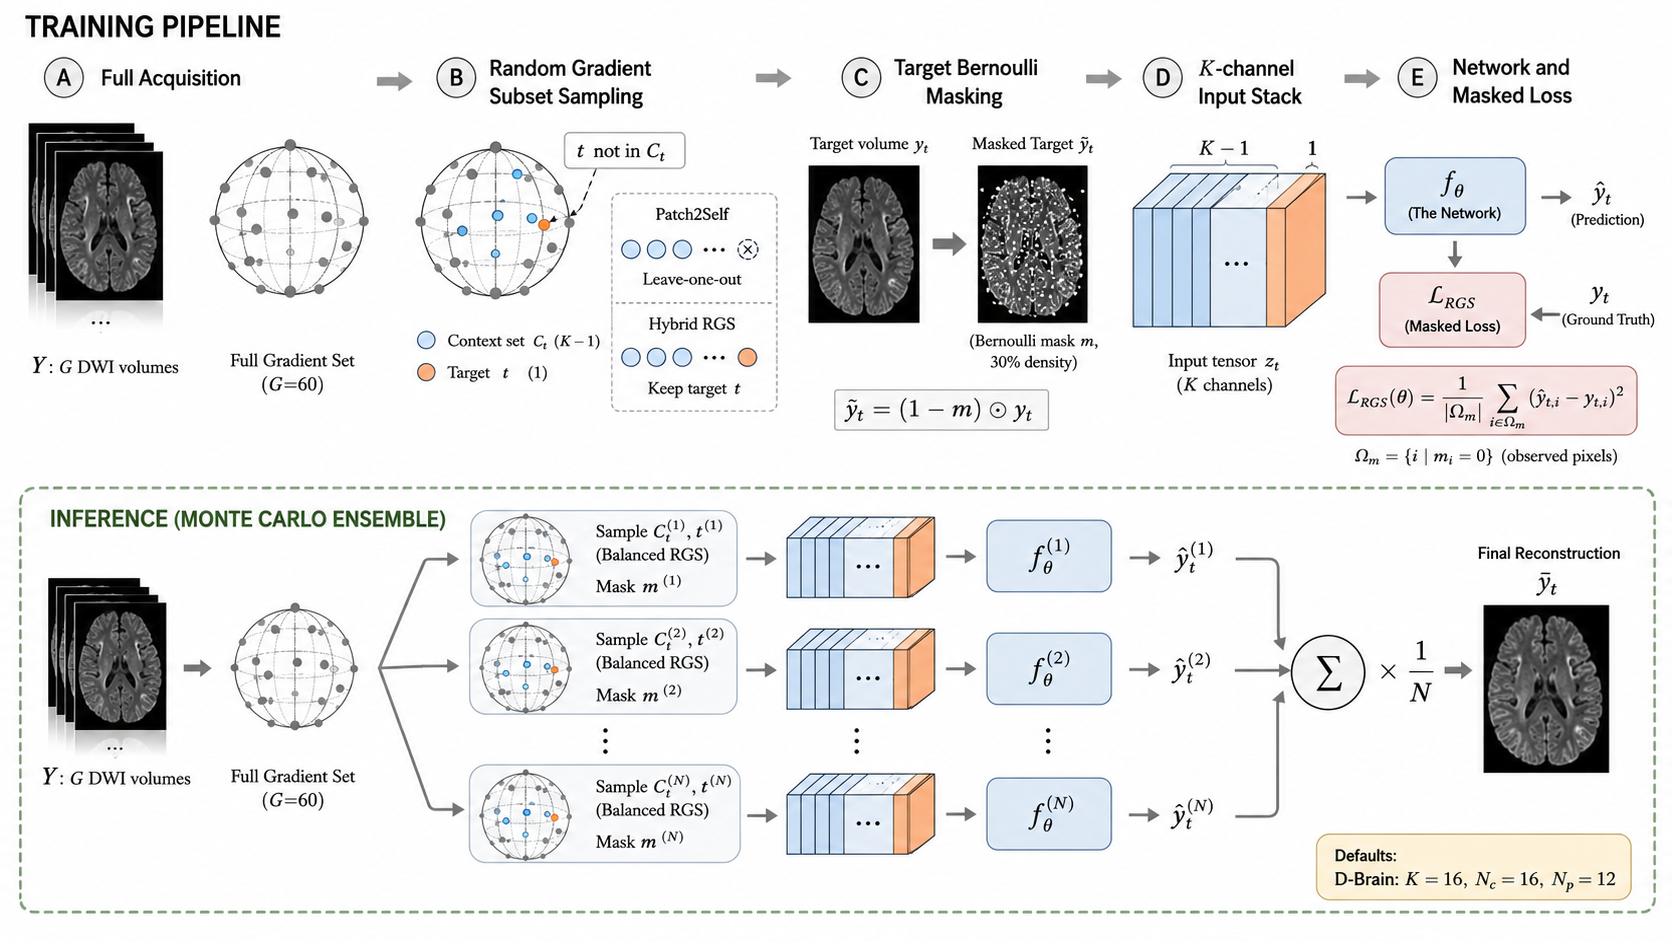
\includegraphics[width=\linewidth]{figures/hybrid_rgs_description.png}
  \caption{Hybrid RGS training and inference pipeline. \textbf{Training (top):} From $G$ diffusion-weighted volumes, a target volume $t$ and context set $C_t$ of $K-1$ gradients are randomly sampled. The context volumes remain unmasked while the target undergoes Bernoulli masking ($p=0.3$) to create $\tilde{y}_t$. These are concatenated into a $K$-channel input stack $z_t$ (target at channel $K-1$) and processed by the denoiser $f_\theta$ (DRCNet or Restormer). The self-supervised loss in Equation~\eqref{eq:rgs-loss} is computed only on masked voxel locations $\Omega_m$, enforcing a blind-spot objective at supervised masked sites; the J-invariance guarantee applies to the training loss at those locations, not to every voxel of the final reconstruction. \textbf{Inference (bottom, dashed):} Each target volume is reconstructed through Monte Carlo ensemble averaging. For $N_c$ random context draws and $N_p$ spatial mask realizations per context, the model generates $N_c \times N_p$ predictions which are averaged to produce the final reconstruction $\bar{y}_t$ in Equation~\eqref{eq:inference-ensemble}. This ensemble is a stochastic masked ensemble rather than a strictly voxel-wise J-invariant estimator, because each voxel is unmasked in many ensemble members. Default D-Brain configuration: $K=16$, $N_c=16$, $N_p=12$; Stanford HARDI: $N_p=23$.}
  \label{fig:hybrid_rgs_pipeline}
\end{figure}

\subsection{J-Invariance of Patch2Self, MD-S2S, and Hybrid RGS}
\todo[author=FHS, color=cyan]{new 2026-07-20 Rewritten}
In the standard Noise2Self setting, let $Y=X+\varepsilon$ denote a noisy observation of an unknown clean signal \cite{jinvariance}. Let $\mathcal{I}$ be the set of signal indices, and let $\mathcal{J}$ be a partition of $\mathcal{I}$. A denoiser $f$ is J-invariant with respect to $\mathcal{J}$ if, for every $J\in\mathcal{J}$, its output on $J$ depends only on the observations outside $J$:
\begin{equation}
  f(y)_J=f(y')_J
  \quad\text{whenever}\quad
  y_{J^c}=y'_{J^c}.
  \label{eq:j-invariance-definition}
\end{equation}
Thus, changing the noisy values in $J$ while keeping their complement fixed cannot change the prediction on $J$. If the noise is conditionally mean-zero and the noise components indexed by $J$ are conditionally independent of those indexed by $J^c$ given $X$, then a J-invariant predictor satisfies the squared-error identity
\begin{equation}
  \mathbb{E}\!\left[\lVert f(Y)-Y\rVert_2^2\right]
  =
  \mathbb{E}\!\left[\lVert f(Y)-X\rVert_2^2\right]
  +
  \mathbb{E}\!\left[\lVert Y-X\rVert_2^2\right].
  \label{eq:j-invariant-risk}
\end{equation}
The final term does not depend on $f$; therefore, minimizing the noisy-target loss is equivalent to minimizing the supervised mean-squared error under these assumptions. Equation~\eqref{eq:j-invariant-risk} is stronger than the structural definition in Equation~\eqref{eq:j-invariance-definition}: a model may be structurally J-invariant even when correlated or biased noise violates the assumptions required for exact risk equivalence. In particular, magnitude-domain Rician observations, such as those generated by Equation~\eqref{eq:rician-noise}, are biased and are not exactly described by conditionally mean-zero additive noise. The J-invariant construction still prevents the direct copying of held-out observations, but its denoising benefit under Rician noise must be established empirically rather than inferred solely from Equation~\eqref{eq:j-invariant-risk}.

\paragraph{Patch2Self.}
Patch2Self uses entire diffusion volumes as the blocks of the J-partition \cite{fadnavis2020patch2self}. For a target volume $t$, let $Y_{-t}$ denote all diffusion-weighted volumes except $Y_t$. Its prediction has the form
\begin{equation}
  \widehat{X}^{\mathrm{P2S}}_t(y_t,Y_{-t})
  =
  \Phi_t(Y_{-t})
  =
  \widehat{X}^{\mathrm{P2S}}_t(y'_t,Y_{-t}).
  \label{eq:patch2self-j-invariance}
\end{equation}
Because the observed target volume is excluded from the predictor inputs, changing $y_t$ while holding $Y_{-t}$ fixed cannot change the output of a fixed fitted regressor. Patch2Self therefore has a strictly volume-wise J-invariant prediction rule, and its inference prediction never receives the target volume as an input. Its interpretation through Equation~\eqref{eq:j-invariant-risk}, however, additionally requires the target-volume noise to be conditionally independent of the noise in the predictor volumes; correlated reconstruction artifacts or motion-related errors may violate this assumption.

\paragraph{MD-S2S and Self2Self.}
MD-S2S extends masking-based self-supervision to multidimensional MRI data \cite{kang2024mds2s}, following the same basic blind-spot principle as Self2Self \cite{self2self}. Using the mask convention of Equation~\eqref{eq:masked-target}, let $\Omega_m=\{i:m_i=1\}$ be the held-out coordinates. A representative masked objective is
\begin{equation}
  \mathcal{L}_{\mathrm{mask}}(\theta)
  =
  \mathbb{E}_{m}\!\left[
    \frac{1}{|\Omega_m|}
    \sum_{i\in\Omega_m}
    \left(
      f_\theta\!\left((1-m)\odot Y\right)_i-Y_i
    \right)^2
  \right].
  \label{eq:masked-self-supervised-loss}
\end{equation}
For any fixed mask, the network input is unchanged if only the held-out values $Y_{\Omega_m}$ are altered; consequently, the predictions evaluated by the loss are J-invariant with respect to $\Omega_m$. Self2Self combines Bernoulli masking with dropout-based model stochasticity, whereas MD-S2S uses random masking over multidimensional MRI data. Their published inference procedures average complete predictions from multiple masked inputs, which can be written generically as
\begin{equation}
  \overline{X}_{\mathrm{mask}}
  =
  \frac{1}{N}
  \sum_{n=1}^{N}
  f_{\theta,\xi_n}\!\left((1-m^{(n)})\odot Y\right),
  \label{eq:masked-ensemble-inference}
\end{equation}
where $\xi_n$ represents additional stochasticity, such as test-time dropout in Self2Self, and may be omitted for deterministic networks. Each ensemble member is blind at the coordinates for which $m_i^{(n)}=1$. However, because a coordinate may be visible in other ensemble members, the averaged image in Equation~\eqref{eq:masked-ensemble-inference} is not necessarily strictly J-invariant at every output coordinate. The training objective is strictly blind at its supervised sites, but the usual full-prediction ensemble relaxes this constraint during inference.

\paragraph{Hybrid RGS.}
Hybrid RGS combines Patch2Self-like exclusion of the target from the angular context with MD-S2S/Self2Self-like masking within the target volume. For a context set $C_t$ satisfying $t\notin C_t$ and a mask $m$, define the prediction at target voxel $i$ as
\begin{equation}
  h_{\theta,t,i}^{C_t,m}(Y)
  =
  f_\theta\!\left(
    \operatorname{concat}\!\left(Y_{C_t},(1-m)\odot Y_t\right)
  \right)_i.
  \label{eq:hybrid-site-prediction}
\end{equation}
For every supervised voxel $i\in\Omega_m$, the value $Y_{t,i}$ is absent from the masked target channel, and the complete target volume is absent from the context channels. Let $Y_{\setminus(t,i)}$ denote all observations except $Y_{t,i}$. Then
\begin{equation}
  h_{\theta,t,i}^{C_t,m}(Y_{t,i},Y_{\setminus(t,i)})
  =
  h_{\theta,t,i}^{C_t,m}(Y'_{t,i},Y_{\setminus(t,i)}),
  \qquad i\in\Omega_m,
  \label{eq:hybrid-j-invariance}
\end{equation}
which directly satisfies Equation~\eqref{eq:j-invariance-definition} for the masked target site $(t,i)$, given fixed model parameters, context, and mask. Equation~\eqref{eq:rgs-loss} evaluates only these sites. Hybrid RGS is therefore structurally J-invariant at the supervised masked voxels for every sampled context and mask. It is not volume-wise J-invariant in the Patch2Self sense because unmasked voxels from the target volume remain available as spatial context. As with the preceding methods, the exact risk identity additionally assumes that the noise at a held-out target voxel is conditionally independent of the noise in the visible target voxels and non-target context volumes.

The reported inference estimator in Equation~\eqref{eq:inference-ensemble} averages complete predictions, including predictions made when voxel $i$ is visible. It therefore has the same inference-time qualification as the usual MD-S2S and Self2Self ensembles: each masked prediction is J-invariant at its held-out sites, but the final full-volume average is not strictly voxel-wise J-invariant everywhere. A strictly J-invariant alternative would retain only predictions for which the reconstructed voxel was masked:
\begin{equation}
  \overline{y}^{\mathrm{strict}}_{t,i}
  =
  \frac{
    \displaystyle\sum_{a=1}^{N_c}\sum_{b=1}^{N_p}
    m_i^{(a,b)} f_\theta\!\left(z_t^{(a,b)}\right)_i
  }{
    \displaystyle\sum_{a=1}^{N_c}\sum_{b=1}^{N_p}m_i^{(a,b)}
  },
  \label{eq:strict-masked-inference}
\end{equation}
provided that the denominator is nonzero. This masked-only estimator would preserve voxel-wise J-invariance at inference, but it would average fewer predictions per voxel and could therefore have higher Monte Carlo variance. The current implementation instead uses the full-prediction ensemble in Equation~\eqref{eq:inference-ensemble}, thereby using more predictions per voxel at the cost of strict voxel-wise J-invariance.

The size and structure of the J-set induce a bias--variance tradeoff. Masking too much target information removes useful spatial context and can increase estimator bias, whereas masking too little weakens the blind-spot constraint and may encourage identity-like behavior. In Hybrid RGS, the masking probability $p$ controls the expected size of the spatial J-set. The subset size $K$ does not change which target voxels belong to the J-set; instead, it controls the amount of non-target angular context available for predicting them. Likewise, the inference parameters $N_c$ and $N_p$ do not alter the training J-set; they control the number of stochastic predictions averaged and, consequently, the Monte Carlo variance of the final reconstruction.

\subsection{Architecture-Agnostic Instantiations}
\label{subsec:architectures}
Hybrid RGS defines the gradient-subset sampling, target masking, $K$-channel input, single-channel output, masked loss, and Monte Carlo inference procedure independently of the denoising backbone. We therefore treat the architectures below as representative instantiations spanning recurrent convolutional, transformer-style, slice-wise, and volumetric models, rather than as separate proposed methods. Unless otherwise stated, all instantiations share the same sampling, masking, loss, and optimization settings; only dimensionality-specific patch shapes and memory-dependent batch sizes differ.

\subsubsection{DRCNet Instantiation}
DRCNet provides a compact recurrent-convolutional 3D instantiation of Hybrid RGS. The model retains the original single-level encoder--decoder and Recurrent Convolutional Denoising Block (RCDB) \cite{gurrola2024drcnet}. The RCDB performs four recurrent refinements and uses parallel $3\times1\times1$, $1\times3\times1$, and $1\times1\times3$ factorized convolutions fused by a $1\times1\times1$ convolution. This configuration preserves the recurrent inductive bias of DRCNet while remaining practical for volumetric patches.

The adaptation is limited primarily to the Hybrid RGS input--output interface. The network receives $K$ channels containing the randomly sampled gradient context and masked target but produces one denoised target channel; consequently, the original global input residual is undefined and is removed. The feature width is reduced from 64 to 32 maps to control memory use, and the output activation is either PReLU or sigmoid. Optional FiLM conditioning is applied at the bottleneck and decoder using the target-gradient metadata vector $[\cos_x,\cos_y,\cos_z,b_{\mathrm{norm}}]$ \cite{perez2018film}. The resulting model contains approximately 0.116M parameters at $K=16$ (Table~\ref{tab:sampling_ablations}). Figure~\ref{fig:drcnet_architecture} summarizes DRCNet3D alongside the independent Plain-CNN-2D comparison architecture.

\begin{figure}[H]
  \centering
  \footnotesize
  \resizebox{0.60\linewidth}{!}{%
    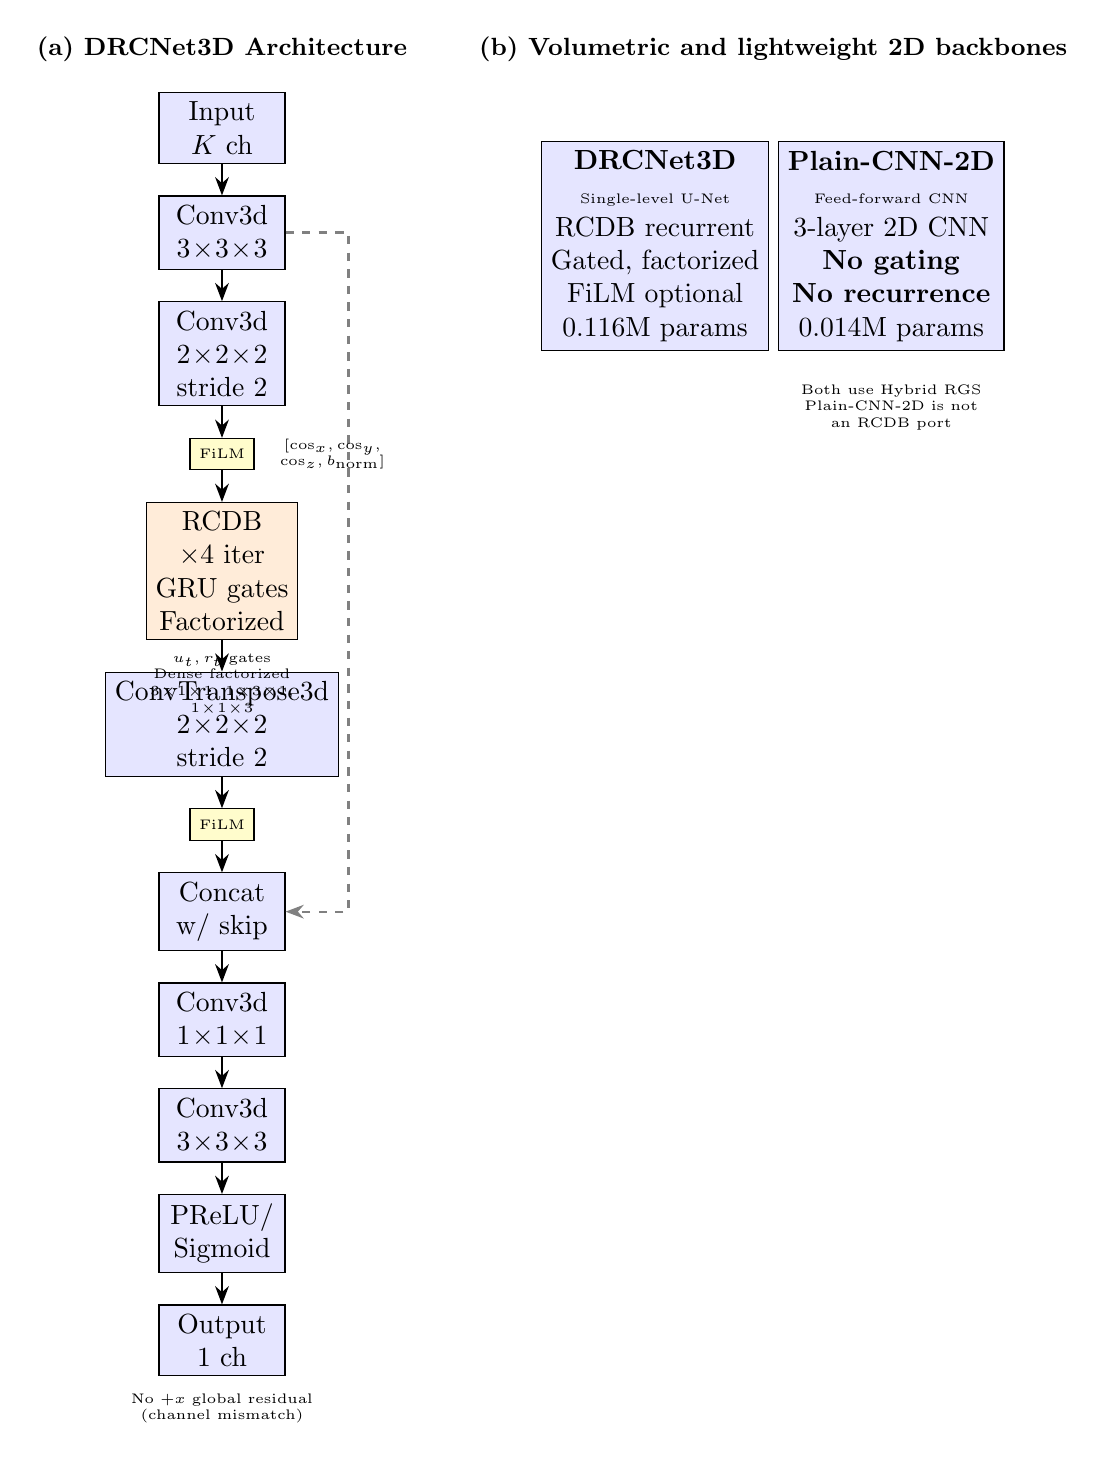
\begin{tikzpicture}[
        node distance=0.5cm and 0.8cm,
        block/.style={rectangle, draw, minimum width=1.6cm, minimum height=0.6cm, align=center, fill=blue!10},
        proc/.style={rectangle, draw, minimum width=1.8cm, minimum height=1.0cm, align=center, fill=orange!15},
        skip/.style={->, thick, dashed, gray, bend right=30},
        >=Stealth
      ]

      % Panel (a) - DRCNet3D architecture
      \node[font=\small\bfseries] at (-3.5, 4.0) {(a) DRCNet3D Architecture};

      % Input
      \node[block] (input) at (-3.5, 3.0) {Input\\$K$ ch};

      % Encoder
      \node[block, below=0.4cm of input] (enc_conv) {Conv3d\\$3\!\times\!3\!\times\!3$};
      \node[block, below=0.4cm of enc_conv] (down) {Conv3d\\$2\!\times\!2\!\times\!2$\\stride 2};

      % FiLM at bottleneck
      \node[block, below=0.4cm of down, fill=yellow!20, minimum width=0.8cm, minimum height=0.4cm, font=\tiny] (film1) {FiLM};

      % RCDB recurrent loop
      \node[proc, below=0.4cm of film1] (rcdb) {RCDB\\$\times 4$ iter\\GRU gates\\Factorized};

      % Skip connection from encoder
      \node[coordinate, right=1.5cm of enc_conv] (skip_point) {};

      % Decoder
      \node[block, below=0.4cm of rcdb] (up) {ConvTranspose3d\\$2\!\times\!2\!\times\!2$\\stride 2};

      % FiLM at decoder
      \node[block, below=0.4cm of up, fill=yellow!20, minimum width=0.8cm, minimum height=0.4cm, font=\tiny] (film2) {FiLM};

      % Concatenation
      \node[block, below=0.4cm of film2] (concat) {Concat\\w/ skip};

      % Output
      \node[block, below=0.4cm of concat] (out_conv1) {Conv3d\\$1\!\times\!1\!\times\!1$};
      \node[block, below=0.4cm of out_conv1] (out_conv2) {Conv3d\\$3\!\times\!3\!\times\!3$};
      \node[block, below=0.4cm of out_conv2] (out_act) {PReLU/\\Sigmoid};
      \node[block, below=0.4cm of out_act] (output) {Output\\$1$ ch};

      % Connections
      \draw[->, thick] (input) -- (enc_conv);
      \draw[->, thick] (enc_conv) -- (down);
      \draw[->, thick] (down) -- (film1);
      \draw[->, thick] (film1) -- (rcdb);
      \draw[->, thick] (rcdb) -- (up);
      \draw[->, thick] (up) -- (film2);
      \draw[->, thick] (film2) -- (concat);
      \draw[->, thick] (concat) -- (out_conv1);
      \draw[->, thick] (out_conv1) -- (out_conv2);
      \draw[->, thick] (out_conv2) -- (out_act);
      \draw[->, thick] (out_act) -- (output);

      % Skip connection
      \draw[->, thick, dashed, gray] (enc_conv.east) -- ++(0.8,0) |- (concat.east);

      % Note about no global residual
      \node[below=0.1cm of output, font=\tiny, align=center, text width=3cm] {No $+x$ global residual\\(channel mismatch)};

      % FiLM annotation
      \node[right=0.2cm of film1, font=\tiny, align=center] {$[\cos_x, \cos_y,$\\$\cos_z, b_{\text{norm}}]$};

      % RCDB detail inset
      \node[below=0.05cm of rcdb, font=\tiny, align=center] {$u_t, r_t$ gates\\Dense factorized\\$3\!\times\!1\!\times\!1$, $1\!\times\!3\!\times\!1$,\\$1\!\times\!1\!\times\!3$};

      % Panel (b) - Volumetric backbone vs lightweight 2D baseline
      \node[font=\small\bfseries] at (3.5, 4.0) {(b) Volumetric and lightweight 2D backbones};

      \node[block, minimum width=2.5cm, minimum height=1.8cm] (drc3d) at (2.0, 1.5) {
        \textbf{DRCNet3D}\\
        \tiny Single-level U-Net\\
        RCDB recurrent\\
        Gated, factorized\\
        FiLM optional\\
        0.116M params
      };

      \node[block, minimum width=2.5cm, minimum height=1.8cm] (drc2d) at (5.0, 1.5) {
        \textbf{Plain-CNN-2D}\\
        \tiny Feed-forward CNN\\
        3-layer 2D CNN\\
        \textbf{No gating}\\
        \textbf{No recurrence}\\
        0.014M params
      };

      \node[below=0.3cm of drc2d, font=\tiny, align=center, text width=2.8cm] {Both use Hybrid RGS\\Plain-CNN-2D is not\\an RCDB port};

    \end{tikzpicture}%
  }% end resizebox
  \caption{Convolutional backbone instantiations under the same Hybrid RGS interface. \textbf{(a)} DRCNet3D uses a single-level encoder--decoder and four RCDB recurrent refinements with factorized 3D convolutions. The $K$-input, one-output-channel interface removes the original global residual, and optional FiLM conditions the bottleneck and decoder. \textbf{(b)} Plain-CNN-2D is an independent three-layer feed-forward baseline without gating or recurrence. The models contain 0.116M and 0.014M parameters, respectively (Tables~\ref{tab:sampling_ablations} and~\ref{tab:3d_vs_2d}).}
  \label{fig:drcnet_architecture}
\end{figure}

\subsubsection{Restormer Instantiation}
Restormer provides a transformer-style counterpart for testing whether Hybrid RGS transfers beyond recurrent convolutional networks \cite{restormer}. The original two-dimensional MDTA and GDFN blocks are extended to volumetric features, while the hierarchy is reduced to three levels to satisfy memory constraints. The baseline uses channel widths of 12, 24, and 48; transformer-block counts of $(1,2,2)$; attention-head counts of $(1,2,2)$; a feed-forward expansion factor of 1.5; and two refinement blocks. Strided and transposed 3D convolutions replace the original PixelUnshuffle and PixelShuffle resampling operations.

As in the DRCNet instantiation, the model receives $K$ input channels and produces one target channel, so the original global input residual is removed. A learned affine output transformation is followed by sigmoid or PReLU activation. Optional FiLM layers condition three intermediate stages on the target-gradient metadata. The baseline model contains approximately 0.178M parameters and follows the same Hybrid RGS training protocol as DRCNet (Table~\ref{tab:3d_vs_2d}). Figure~\ref{fig:restormer3d_arch} summarizes the architecture.

A larger Restormer3D configuration is included only as a capacity-control experiment. It preserves the same three-level topology and Hybrid RGS protocol while increasing the embedding width from 12 to 24, the block counts from $(1,2,2)$ to $(2,4,10)$, the attention-head counts from $(1,2,2)$ to $(1,2,4)$, the feed-forward expansion factor from 1.5 to 2.66, and the refinement depth from two to four blocks. This model contains approximately 2.10M parameters and is used to distinguish the effect of backbone capacity from that of spatial dimensionality (Table~\ref{tab:3d_vs_2d}).

\subsubsection{Two-Dimensional Backbones for Architecture Evaluation}
\todo[author=FHS, color=cyan]{new 2026-07-14 Original Restormer 2D vs 3D vs other backbones}
The architecture evaluation (Section~\ref{subsec:capacity_dimensionality}, Table~\ref{tab:3d_vs_2d}) uses three slice-wise backbones. Plain-CNN-2D and Res-CNN-2D are deliberately small, independent convolutional models used to test whether Hybrid RGS works with inexpensive 2D architectures. Restormer-2D follows the original two-dimensional Restormer formulation and is approximately capacity matched to Restormer3D, providing the only controlled dimensionality comparison in this group.

Plain-CNN-2D contains three convolutional layers with PReLU activation and no recurrence, gating, attention, or skip connections. Res-CNN-2D uses a convolutional embedding, lightweight residual blocks with GELU activation, and a single-channel output projection. They contain approximately 0.014M and 0.015M parameters, respectively, and are intended as minimal baselines rather than two-dimensional ports of DRCNet or Restormer. In particular, Plain-CNN-2D is distinct from the recurrent DRCNet-2D architecture of Gurrola et al. \cite{gurrola2024drcnet}.

Restormer-2D retains the same baseline widths, block counts, attention heads, feed-forward expansion, and refinement depth as Restormer3D while using the original two-dimensional MDTA/GDFN blocks and PixelShuffle-based resampling \cite{restormer}. It contains approximately 0.149M parameters, compared with 0.178M for Restormer3D, and provides the controlled within-family dimensionality comparison shown in Figure~\ref{fig:backbone_comparison}.

All 2D backbones use the same random gradient subsets, Bernoulli masking probability $p=0.3$, masked loss, optimizer, and progressive in-plane patch schedule. They process axial slices independently and receive no through-plane context. Comparisons involving Plain-CNN-2D or Res-CNN-2D jointly change architecture, capacity, and dimensionality, whereas Restormer-2D versus Restormer3D approximately controls architecture and capacity to isolate spatial dimensionality.

\begin{figure}[H]
  \centering
  \footnotesize
  \resizebox{0.42\linewidth}{!}{%
    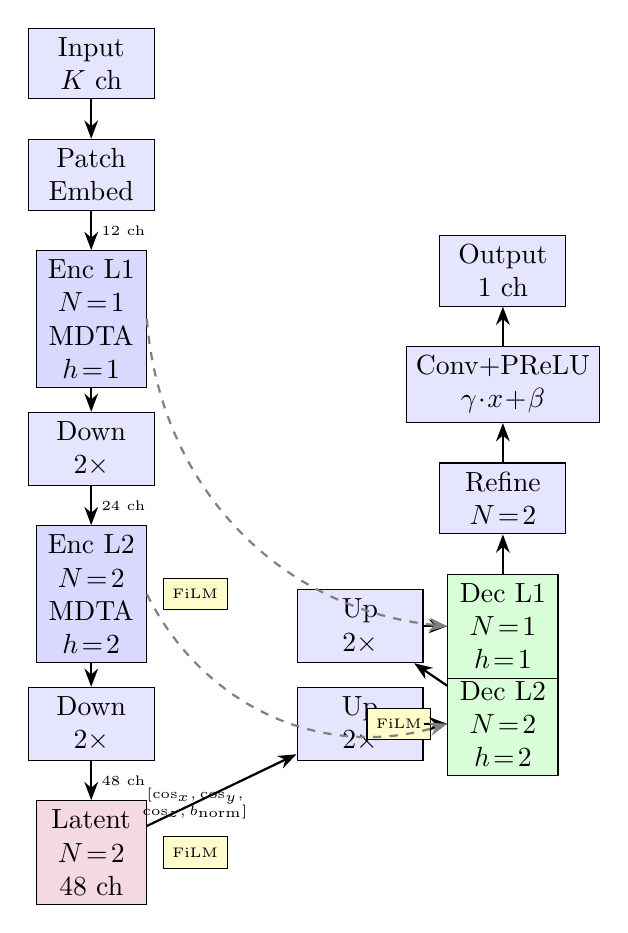
\begin{tikzpicture}[
        node distance=0.5cm and 0.8cm,
        block/.style={rectangle, draw, minimum width=1.6cm, minimum height=0.6cm, align=center, fill=blue!10},
        enc/.style={rectangle, draw, minimum width=1.4cm, minimum height=1.2cm, align=center, fill=blue!15},
        dec/.style={rectangle, draw, minimum width=1.4cm, minimum height=1.2cm, align=center, fill=green!15},
        skip/.style={->, thick, dashed, gray, bend right=40},
        >=Stealth
      ]

      % Input
      \node[block] (input) at (0, 2.5) {Input\\$K$ ch};
      \node[block, below=of input] (embed) {Patch\\Embed};

      % Encoder
      \node[enc, below=of embed] (enc1) {Enc L1\\$N\!=\!1$\\MDTA\\$h\!=\!1$};
      \node[block, below=0.3cm of enc1] (down1) {Down\\$2\times$};
      \node[enc, below=of down1] (enc2) {Enc L2\\$N\!=\!2$\\MDTA\\$h\!=\!2$};
      \node[block, right=0.2cm of enc2, fill=yellow!20, minimum width=0.8cm, minimum height=0.4cm, font=\tiny] (film1) {FiLM};
      \node[block, below=0.3cm of enc2] (down2) {Down\\$2\times$};

      % Bottleneck
      \node[enc, below=of down2, fill=purple!15] (latent) {Latent\\$N\!=\!2$\\48 ch};
      \node[block, right=0.2cm of latent, fill=yellow!20, minimum width=0.8cm, minimum height=0.4cm, font=\tiny] (film2) {FiLM};

      % Decoder
      \node[block, right=1.8cm of down2] (up2) {Up\\$2\times$};
      \node[dec, right=0.3cm of up2] (dec2) {Dec L2\\$N\!=\!2$\\$h\!=\!2$};
      \node[block, left=0.2cm of dec2, fill=yellow!20, minimum width=0.8cm, minimum height=0.4cm, font=\tiny] (film3) {FiLM};
      \node[block, right=1.8cm of down1, above=0.3cm of up2] (up1) {Up\\$2\times$};
      \node[dec, right=0.3cm of up1] (dec1) {Dec L1\\$N\!=\!1$\\$h\!=\!1$};

      % Output
      \node[block, above=of dec1] (refine) {Refine\\$N\!=\!2$};
      \node[block, above=of refine] (output) {Conv+PReLU\\$\gamma\!\cdot\!x\!+\!\beta$};
      \node[block, above=of output] (out) {Output\\$1$ ch};

      % Connections
      \draw[->, thick] (input) -- (embed);
      \draw[->, thick] (embed) -- (enc1) node[midway, right, font=\tiny] {12 ch};
      \draw[->, thick] (enc1) -- (down1);
      \draw[->, thick] (down1) -- (enc2) node[midway, right, font=\tiny] {24 ch};
      \draw[->, thick] (enc2) -- (down2);
      \draw[->, thick] (down2) -- (latent) node[midway, right, font=\tiny] {48 ch};
      \draw[->, thick] (latent) -- (up2);
      \draw[->, thick] (up2) -- (dec2);
      \draw[->, thick] (dec2) -- (up1);
      \draw[->, thick] (up1) -- (dec1);
      \draw[->, thick] (dec1) -- (refine);
      \draw[->, thick] (refine) -- (output);
      \draw[->, thick] (output) -- (out);

      % Skip connections
      \draw[skip] (enc1.east) to (dec1.west);
      \draw[skip] (enc2.east) to (dec2.west);

      % FiLM annotation
      \node[above=0.1cm of film2, font=\tiny, align=center] {$[\cos_x, \cos_y,$\\$\cos_z, b_{\text{norm}}]$};

    \end{tikzpicture}%
  }% end resizebox
  \caption{Transformer-style backbone instantiations under Hybrid RGS. Restormer3D uses a three-level encoder--decoder with volumetric MDTA and GDFN blocks, channel widths of 12, 24, and 48, skip connections, refinement blocks, and a learned affine output head. Optional FiLM layers (yellow) condition three stages on the target-gradient metadata. Restormer-2D follows the original two-dimensional Restormer formulation, using 2D MDTA/GDFN blocks and PixelUnshuffle/PixelShuffle resampling with approximately matched baseline topology and capacity.}
  \label{fig:restormer3d_arch}
\end{figure}

\begin{figure}[H]
  \centering
  \footnotesize
  \todo[author=FHS, color=cyan, inline]{new 2026-07-14 Original Restormer 2D vs 3D vs other backbones}
  \resizebox{\linewidth}{!}{%
    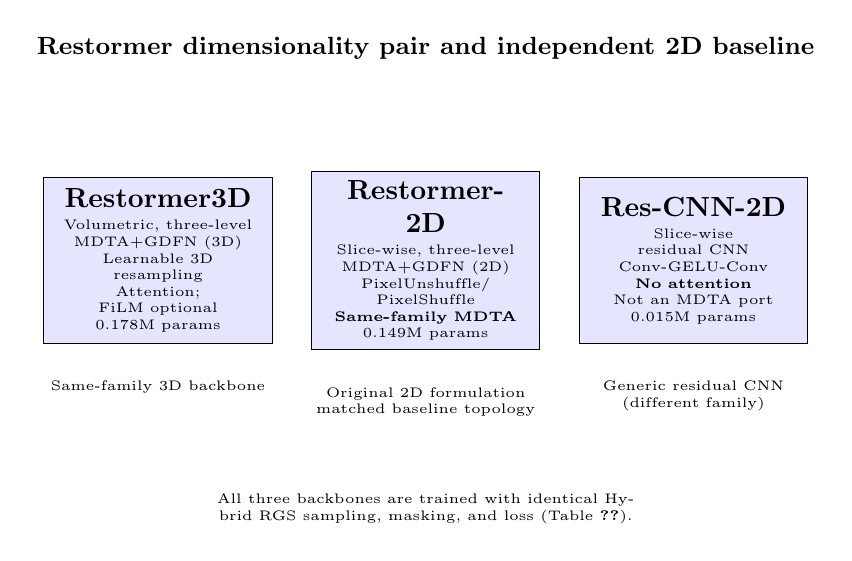
\begin{tikzpicture}[
        node distance=0.5cm and 0.8cm,
        block/.style={rectangle, draw, minimum width=1.6cm, minimum height=0.6cm, align=center, fill=blue!10},
        >=Stealth
      ]

      \node[font=\small\bfseries] at (3.4, 2.7) {Restormer dimensionality pair and independent 2D baseline};

      \node[block, minimum width=2.9cm, minimum height=2.1cm, text width=2.5cm, font=\tiny] (rest3d) at (0, 0) {
        \normalsize\textbf{Restormer3D}\\[2pt]
        \tiny Volumetric, three-level\\
        MDTA+GDFN (3D)\\
        Learnable 3D resampling\\
        Attention; FiLM optional\\
        0.178M params
      };

      \node[block, minimum width=2.9cm, minimum height=2.1cm, text width=2.5cm, font=\tiny] (rest2d) at (3.4, 0) {
        \normalsize\textbf{Restormer-2D}\\[2pt]
        \tiny Slice-wise, three-level\\
        MDTA+GDFN (2D)\\
        PixelUnshuffle/\\
        PixelShuffle\\
        \textbf{Same-family MDTA}\\
        0.149M params
      };

      \node[block, minimum width=2.9cm, minimum height=2.1cm, text width=2.5cm, font=\tiny] (rescnn2d) at (6.8, 0) {
        \normalsize\textbf{Res-CNN-2D}\\[2pt]
        \tiny Slice-wise residual CNN\\
        Conv-GELU-Conv\\
        \textbf{No attention}\\
        Not an MDTA port\\
        0.015M params
      };

      \node[below=0.35cm of rest3d, font=\tiny, align=center, text width=2.9cm] {Same-family 3D backbone};
      \node[below=0.35cm of rest2d, font=\tiny, align=center, text width=2.9cm] {Original 2D formulation\\matched baseline topology};
      \node[below=0.35cm of rescnn2d, font=\tiny, align=center, text width=2.9cm] {Generic residual CNN\\(different family)};

      \node[below=1.7cm of rest2d, font=\tiny, align=center, text width=9.5cm] {All three backbones are trained with identical Hybrid RGS sampling, masking, and loss (Table~\ref{tab:3d_vs_2d}).};

    \end{tikzpicture}%
  }% end resizebox
  \caption{Backbones used in the architecture evaluation. Restormer3D and the original Restormer-2D formulation form an approximately capacity-matched pair for testing volumetric versus slice-wise processing within the Restormer family. Res-CNN-2D is an independent, much smaller residual architecture that tests whether Hybrid RGS remains effective with limited model capacity. All three use the same gradient sampling, target masking, and self-supervised loss (Table~\ref{tab:3d_vs_2d}).}
  \label{fig:backbone_comparison}
\end{figure}

\subsection{Inference}
At inference, each target volume is reconstructed using the stochastic ensemble procedure shown at the bottom of Figure~\ref{fig:hybrid_rgs_pipeline}. For target volume $t$, the method samples $N_c$ random context sets $C_t^{(1)},\ldots,C_t^{(N_c)}$ from the non-target gradients. For each context, $N_p$ spatial masks are drawn independently, producing $N_p$ masked inputs and corresponding full-volume predictions. The final reconstruction is their average:
\begin{equation}
  \bar{y}_t =
  \frac{1}{N_c N_p}
  \sum_{a=1}^{N_c}\sum_{b=1}^{N_p}
  f_\theta\left(z_t^{(a,b)}\right),
  \label{eq:inference-ensemble}
\end{equation}
where $z_t^{(a,b)}$ denotes the input formed from context $C_t^{(a)}$ and spatial mask $m^{(a,b)}$, and $f_\theta$ is the trained denoiser. This procedure performs Monte Carlo ensembling over both random angular contexts and Bernoulli masks of the target channel. Unlike a masked-voxel-only estimator, which would preserve strict per-voxel J-invariance during inference, the reported implementation averages complete volume predictions. It therefore uses more predictions per voxel and is intended to reduce Monte Carlo variance, but it may include predictions obtained when a voxel is visible in the target channel. The output should consequently be interpreted as a stochastic masked ensemble rather than as a strictly voxel-wise J-invariant estimator.

Unless otherwise stated, the D-Brain experiments use $N_c=16$ context samples and $N_p=12$ spatial mask draws per context, totaling 192 forward passes per target volume. The reported Stanford HARDI protocol uses $N_c=16$ and $N_p=23$. Reconstructing all $G$ target volumes therefore requires $G N_c N_p$ forward passes, so inference cost grows linearly with the number of gradients and both ensemble dimensions.

\section{Experiments}
\subsection{Datasets and Protocols}
The primary experiments use the D-Brain and Stanford HARDI datasets. Synthetic Rician noise is added to the clean D-Brain phantom, enabling direct evaluation of PSNR, SSIM, and tensor-derived metrics. Stanford HARDI is used to assess feasibility on real scanner data under a different acquisition protocol, without clean ground truth.

For synthetic D-Brain experiments, noise is added after per-volume min--max normalization. For each voxel with clean normalized signal $s \in [0,1]$ and noise level $\sigma$, the corrupted magnitude is
\begin{equation}
  y = \sqrt{(s + \eta_1)^2 + \eta_2^2},
  \qquad \eta_1,\eta_2 \sim \mathcal{N}(0,\sigma^2),
  \label{eq:rician-noise}
\end{equation}
where independent Gaussian samples are drawn for every voxel and diffusion volume, and $\sigma$ denotes their standard deviation. The corrupted values are clipped to $[0,1]$. Because the noise samples are independent across voxels and volumes, this synthetic model satisfies the noise-independence assumptions underlying the J-invariant objective at masked locations. The robustness experiments use $\sigma \in \{0.05,0.10,0.15,0.20\}$, with $\sigma=0.10$ as the primary condition.

Image-domain evaluation reports MSE, PSNR, and SSIM over the full 4D array and within a brain-tissue region of interest (ROI). Full-volume metrics include every spatial voxel and diffusion channel. PSNR uses the peak intensity of the clean reference as the dynamic range,
\begin{equation}
  \operatorname{PSNR} = 20\log_{10}\left(\frac{\max(X)}{\sqrt{\operatorname{MSE}}}\right),
  \label{eq:psnr}
\end{equation}
where $X$ denotes the original clean array. SSIM is computed using the scikit-image implementation, with the data range $\max(X)-\min(X)$, the fourth dimension treated as the diffusion-volume channel axis, and the default local-window settings retained \cite{vanderwalt2014skimage}. The evaluation mask is defined as $\Omega_{\mathrm{ROI}}^{\mathrm{eval}}=\{i:\max_g X_i(g)>0.02\}$ and is computed from the clean reference independently of the stochastic Bernoulli training mask $m$. The evaluation mask itself is not used for training-patch selection or checkpoint selection. MSE-ROI and PSNR-ROI are computed using only voxels in $\Omega_{\mathrm{ROI}}^{\mathrm{eval}}$. PSNR-ROI uses the same peak intensity as full-volume PSNR, namely $\max(X)$ over the full clean array. SSIM-ROI is computed on the bounding-box crop enclosing the ROI to preserve local neighborhoods.

Tensor-derived maps are computed with DIPY 1.x \texttt{TensorModel} using ordinary least squares without additional regularization \cite{garyfallidis2014dipy}. Before tensor fitting, the denoised DWI volumes are restored to the original phantom scale using the stored per-volume min--max parameters. The gradient table is constructed from the acquisition $b$-values and $b$-vectors, and the non-diffusion-weighted ($b0$) images, defined by $b\leq50~\mathrm{s/mm^2}$, are combined with the denoised DWI stack.

For \textbf{D-Brain}, FA, MD, AD, and RD maps are computed from each denoised output and compared with the clean phantom ground truth using ROI mean absolute error. For example,
\begin{equation}
  \operatorname{FA\mbox{-}MAE}=\frac{1}{|\Omega_{\mathrm{ROI}}^{\mathrm{eval}}|}\sum_{i\in\Omega_{\mathrm{ROI}}^{\mathrm{eval}}}|\operatorname{FA}_{\mathrm{denoised},i}-\operatorname{FA}_{\mathrm{GT},i}|,
  \label{eq:fa-mae}
\end{equation}
with analogous definitions used for MD-MAE, AD-MAE, and RD-MAE. FA is dimensionless. The diffusivity errors use the units returned by DIPY after restoration to the phantom scale. For D-Brain, these values are relative to the simulation intensity scale and should be compared across methods rather than interpreted as physical diffusivities in $\mathrm{mm^2/s}$.

For \textbf{Stanford HARDI}, no clean ground truth is available. Tensor maps are computed from the denoised outputs and, where reported, compared with an internal reference obtained by fitting the tensor model to the acquired signal before denoising. These comparisons quantify deviation from the input-derived tensor estimate rather than ground-truth error. Accordingly, Stanford results are reported as deviations from the internal reference rather than as MAE.

\subsection{Baselines}
Unless otherwise stated, the external baselines are evaluated using their published formulations and are not modified to incorporate Hybrid RGS. MP-PCA, Patch2Self, and MD-S2S therefore use the full available diffusion acquisition rather than sampled subsets of $K$ volumes. MP-PCA is a non-learning method applied jointly to the diffusion series. Patch2Self performs leave-one-volume-out regression, predicting each target from the remaining $G-1$ volumes, whereas MD-S2S is trained on the full multidimensional dataset using its published masking strategy. Only methods explicitly labeled as Hybrid RGS receive inputs consisting of one masked target and $K-1$ sampled context volumes.

The comparison includes the following external baselines and internal reference models:
\begin{itemize}
  \item the unprocessed noisy input;
  \item MP-PCA as a classical diffusion MRI baseline \cite{veraart2016mppca};
  \item Patch2Self with the DIPY ordinary-least-squares backend \cite{fadnavis2020patch2self};
  \item the two-dimensional MD-S2S masking method \cite{kang2024mds2s};
  \item independent two-dimensional, slice-wise Hybrid RGS backbones used in the architecture evaluation; and
  \item supervised reference models that retain the Hybrid RGS sampling protocol but use clean targets.
\end{itemize}

\subsection{Evaluation Metrics}
\label{subsec:metrics}
Image-domain fidelity is assessed using MSE, PSNR, and SSIM over the full 4D array and within the brain-tissue ROI. Preservation of tensor-derived quantities is evaluated using errors in FA, MD, AD, and RD after tensor fitting. Inference time and model size are reported when available to characterize computational cost.

\subsection{Ablation Studies}
The ablation studies isolate the principal design choices of the framework:
\begin{itemize}
  \item objective-controlled DRCNet variants that separate angular-only, spatial-only, sequential-hybrid, and full Hybrid RGS training;
  \item sequential context selection versus random gradient-subset sampling at the same value of $K$;
  \item variation in $K$, the number of volumes in each sampled input group;
  \item sensitivity to backbone choice across DRCNet-Hybrid-RGS, Restormer-Hybrid-RGS, and lightweight two-dimensional models; and
  \item the effects of backbone capacity and spatial dimensionality, including comparisons between volumetric 3D and slice-wise 2D architectures under the same Hybrid RGS objective.
\end{itemize}
Unless otherwise stated, the D-Brain ablations fix the masking probability at $p=0.3$, the number of inference context samples at $N_c=16$, the number of inference mask draws at $N_p=12$, and the progressive patch schedule. Stanford HARDI uses $N_p=23$, as described above. These settings are not independently varied in the reported ablations.

\subsection{Objective-Controlled Ablation}
The main comparison in Table~\ref{tab:main_comparison} motivates this ablation because the Hybrid RGS models substantially outperform Patch2Self and MD-S2S in image-domain ROI metrics. However, that comparison alone cannot determine whether the gains arise from the DRCNet backbone or from the self-supervised objective. We therefore fix the backbone to the same 3D DRCNet and vary only the training objective. The ablation separates three design axes: the use of angular context from non-target diffusion gradients, spatial masking of the target channel to enforce a blind-spot loss, and random rather than deterministic sampling of the angular context. All four conditions use the same D-Brain data with Rician noise at $\sigma=0.1$, normalization, patching strategy, optimizer, learning rate, training budget, and evaluation protocol.

The first condition, DRCNet Angular-Only, uses a neural, limited-context Patch2Self-style objective. The network receives $K-1$ randomly sampled context gradients that exclude the target volume and predicts the complete target volume using a full-volume loss. Because the target is absent from the input, spatial target masking is unnecessary. This condition tests whether angular redundancy alone is sufficient when a nonlinear DRCNet replaces the linear Patch2Self regressor. The second condition, DRCNet Spatial-Only, uses a volumetric Self2Self-style objective. The network receives only the target volume with Bernoulli-masked voxels and is optimized with a masked loss, without auxiliary diffusion gradients. This condition tests whether spatial context alone can denoise DWI volumes. The third condition, DRCNet Sequential Hybrid, combines a masked target channel with $K-1$ auxiliary gradients selected using a deterministic sequential window. The fourth condition is the proposed DRCNet Hybrid RGS objective, which combines the masked target channel with $K-1$ randomly sampled non-target gradients and evaluates the loss only at masked voxels.

Table~\ref{tab:objective_controlled_ablation} shows that angular context alone is insufficient under the limited input budget used in this experiment. DRCNet Angular-Only reaches $10.87$ dB PSNR-ROI despite using the same neural backbone. When the target volume is excluded from the input, the network must reconstruct it entirely from other diffusion directions. Although these directions share anatomical structure with the target, they do not directly provide its direction-specific contrast and spatial detail, resulting in substantial image-domain degradation.

Importantly, DRCNet Angular-Only uses $K-1=15$ randomly sampled context gradients and contains no target channel. It is therefore a matched-channel-budget ablation rather than a full neural replacement for Patch2Self. Its purpose is to isolate the contribution of target-channel spatial masking while keeping the input dimensionality comparable to Hybrid RGS with $K=16$. A full neural Patch2Self-style model would instead condition on all $G-1=59$ non-target gradients and would require a different input layer, memory budget, and training configuration. Thus, the result demonstrates the limitations of angular-only prediction at the matched channel budget, not of neural Patch2Self-style models in general.

Spatial masking alone performs substantially better. DRCNet Spatial-Only reaches $24.47$ dB PSNR-ROI and the lowest FA-MAE in this ablation, showing that the blind-spot objective can exploit considerable local anatomical structure. It also outperforms DRCNet Sequential Hybrid in PSNR-ROI ($24.47$ versus $23.60$ dB). This result suggests that a fixed angular window does not provide sufficiently diverse context and may encourage dependencies on a particular channel arrangement. Nevertheless, Spatial-Only remains $2.46$ dB below full Hybrid RGS, indicating that angular context is beneficial when coupled with random sampling.

The full DRCNet Hybrid RGS objective achieves the highest image-domain fidelity, with $26.93$ dB PSNR-ROI and $0.5247$ SSIM-ROI. Together with the sequential-versus-random comparison in Table~\ref{tab:sampling_ablations}, the gain over Sequential Hybrid is consistent with random subsets providing angular data augmentation: the model encounters varied diffusion contexts rather than fixed channel neighborhoods. FA-MAE and MD-MAE vary over a narrower range than PSNR-ROI and SSIM-ROI, and Hybrid RGS does not achieve the best FA-MAE; this ablation therefore does not establish tensor-domain superiority. Instead, it shows that, with the DRCNet backbone fixed, Hybrid RGS provides the strongest image reconstruction fidelity among the angular-only, spatial-only, sequential-hybrid, and random-hybrid objectives. The improvement can therefore be attributed to the coupled random-gradient-subset and target-masking scheme rather than to differences in backbone capacity.

\begin{table}[ht]
  \centering
  \caption{Objective-controlled ablation on D-Brain with Rician noise $\sigma=0.1$. All rows use the same DRCNet backbone, training budget, and evaluation protocol. The ablation isolates angular context, target-channel masking, and random gradient-subset sampling.}
  \label{tab:objective_controlled_ablation}
  \resizebox{\linewidth}{!}{%
    \begin{tabular}{lcccccccc}
      \toprule
      Training objective & Angular & Masking & Random context & PSNR-ROI $\uparrow$ & SSIM-ROI $\uparrow$ & FA-MAE $\downarrow$ & MD-MAE$^\dagger$ (a.u.) $\downarrow$ & Time/vol. (s) \\
      \midrule
      DRCNet Angular-Only & \checkmark & -- & \checkmark & 10.87 & 0.3407 & 0.2328 & 3499 & 5.2 \\
      DRCNet Spatial-Only & -- & \checkmark & -- & 24.47 & 0.4778 & \textbf{0.2234} & 3457 & 4.5 \\
      DRCNet Sequential Hybrid & \checkmark & \checkmark & -- & 23.60 & 0.4751 & 0.2390 & 3555 & \textbf{3.7} \\
      DRCNet Hybrid RGS & \checkmark & \checkmark & \checkmark & \textbf{26.93} & \textbf{0.5247} & 0.2575 & \textbf{3451} & 34.1 \\
      \bottomrule
    \end{tabular}
  }
\end{table}
\par\noindent\textit{Note:} $^\dagger$MD-MAE values are reported in arbitrary units derived from the D-Brain phantom intensity scale and should be interpreted as relative comparisons across methods.

\subsection{Sampling Strategy Ablations}
Hybrid RGS uses random gradient subsets rather than locally sequential angular windows. To assess this design choice, we first compare random gradient sampling with a sequential-window strategy using the same number of input channels. The two modes differ as follows.

\textbf{RGS mode.} At each training step, an ordered tuple of $K$ distinct gradient indices is sampled uniformly without replacement from $\{0,\ldots,G-1\}$. The volume at position $K-1$ is designated as the masked target, and the volumes at positions $0,\ldots,K-2$ provide context. Every gradient index has the same probability of being selected as the target at each step, permitting coverage of all target indices over the course of training.

\textbf{Sequential mode.} A window start $s$ is sampled uniformly from $\{0,\ldots,G-K\}$, yielding the indices $s,s+1,\ldots,s+K-1$. The final index, $s+K-1$, is the masked target, and the preceding $K-1$ indices provide context. The possible target indices therefore span $\{K-1,\ldots,G-1\}$; the first $K-1$ gradient indices, $\{0,\ldots,K-2\}$, are never used as targets. This asymmetry follows from the adopted boundary convention and must be considered when interpreting the sequential-versus-random gap. Part of the lower PSNR-ROI in sequential mode may result from incomplete target coverage rather than solely from the absence of diverse, nonlocal angular context.

Both sampling modes are evaluated on D-Brain with Rician noise at $\sigma=0.1$ using $K=16$, the same masking probability, learning rate, patching strategy, and number of epochs. We evaluate both DRCNet and Restormer to test whether the benefit of random angular context is architecture dependent.

The results in Table~\ref{tab:sampling_ablations} show that random sampling improves PSNR-ROI for both backbones. For DRCNet, PSNR-ROI increases from $23.60$ to $26.93$ dB, while FA-MAE worsens from $0.2390$ to $0.2575$. For Restormer, PSNR-ROI increases from $21.64$ to $23.43$ dB and FA-MAE improves from $0.2465$ to $0.2238$. Thus, the image-domain benefit is consistent across architectures, whereas the tensor-domain effect is architecture dependent. These results should not be interpreted as a general failure of sequential windowing: adjacent gradients remain informative, and the blind-spot masking objective is active in both modes. Moreover, the sequential strategy has incomplete target-index coverage under the adopted boundary convention. Subject to this qualification, the PSNR-ROI gains are consistent with RGS providing angular data augmentation by exposing the models to more varied diffusion contexts and reducing reliance on fixed local channel neighborhoods.

A second ablation examines the number of input volumes $K$. A small value limits angular information and may force the network to rely primarily on spatial interpolation. A large value increases memory use, parameter count, and runtime while potentially introducing redundant diffusion measurements. Establishing a practical range for $K$ is important because acquisition protocols vary substantially: D-Brain contains $G=60$ diffusion-weighted volumes, whereas Stanford HARDI contains $G=150$.

We evaluate $K \in \{5,10,16,24,30\}$ on D-Brain under the same noise setting. Each value of $K$ requires a separate model because the input channel dimension changes. DRCNet and Restormer are both evaluated across the full sweep. Within each backbone, all runs use the same core Hybrid RGS protocol and inference-ensemble settings.

The quality curves are non-monotonic and architecture dependent. DRCNet obtains the same PSNR-ROI at $K=5$ and $K=10$ ($26.46$ dB), reaches its maximum at $K=16$ ($26.93$ dB), remains nearly unchanged at $K=24$ ($26.92$ dB), and decreases to $26.36$ dB at $K=30$. Restormer achieves its highest PSNR-ROI at $K=10$ ($26.60$ dB). Its performance drops at $K=16$ ($23.43$ dB) and partially recovers at $K=24$ and $K=30$ ($25.83$ and $25.50$ dB, respectively). These results do not support a single optimal value of $K$ across backbones.

The runtime and model-size trends favor moderate values of $K$. For DRCNet, the parameter count grows from $0.106$M at $K=5$ to $0.128$M at $K=30$, while inference time increases from $32.5$ to $37.2$ s per target volume. Restormer is more expensive overall, with inference times ranging from $126.8$ to $131.9$ s per volume. Although the runtime increase across $K$ is modest in these experiments, larger inputs also increase memory pressure and training cost. We retain $K=16$ as the fixed cross-model operating point because it is optimal for DRCNet and maintains a moderate channel count; it should not be interpreted as universally optimal. The Restormer results instead favor $K=10$, demonstrating the need for backbone-specific selection of $K$.

\begin{table}[ht]
  \centering
  \caption{Sampling ablations on D-Brain with Rician noise $\sigma=0.1$. The first block compares sequential-window and random gradient sampling at $K=16$. The second block summarizes the $K$ sweep. Params and time/vol. are reported when available. Bold indicates the best PSNR-ROI and FA-MAE within each architecture and table block.}
  \label{tab:sampling_ablations}
  \resizebox{\linewidth}{!}{%
    \begin{tabular}{llcccc}
      \toprule
      Architecture & Sampling / $K$ & PSNR-ROI $\uparrow$ & FA-MAE $\downarrow$ & Params (M) & Time/vol. (s) \\
      \midrule
      DRCNet & Sequential, $K=16$ & 23.60 & \textbf{0.2390} & 0.116 & 3.7 \\
      DRCNet & RGS, $K=16$ & \textbf{26.93} & 0.2575 & 0.116 & 34.1 \\
      Restormer & Sequential, $K=16$ & 21.64 & 0.2465 & 0.178 & 104.2 \\
      Restormer & RGS, $K=16$ & \textbf{23.43} & \textbf{0.2238} & 0.178 & 126.8 \\
      \midrule
      DRCNet & RGS, $K=5$ & 26.46 & \textbf{0.2319} & 0.106 & 32.5 \\
      DRCNet & RGS, $K=10$ & 26.46 & 0.2378 & 0.111 & 33.8 \\
      DRCNet & RGS, $K=16$ & \textbf{26.93} & 0.2575 & 0.116 & 34.1 \\
      DRCNet & RGS, $K=24$ & 26.92 & 0.2559 & 0.123 & 36.1 \\
      DRCNet & RGS, $K=30$ & 26.36 & 0.2464 & 0.128 & 37.2 \\
      Restormer & RGS, $K=5$ & 25.88 & 0.2489 & 0.174 & 129.2 \\
      Restormer & RGS, $K=10$ & \textbf{26.60} & \textbf{0.2195} & 0.176 & 129.2 \\
      Restormer & RGS, $K=16$ & 23.43 & 0.2238 & 0.178 & 126.8 \\
      Restormer & RGS, $K=24$ & 25.83 & 0.2198 & 0.180 & 130.2 \\
      Restormer & RGS, $K=30$ & 25.50 & 0.2199 & 0.182 & 131.9 \\
      \bottomrule
    \end{tabular}
  }
\end{table}

\begin{figure}[H]
  \centering
  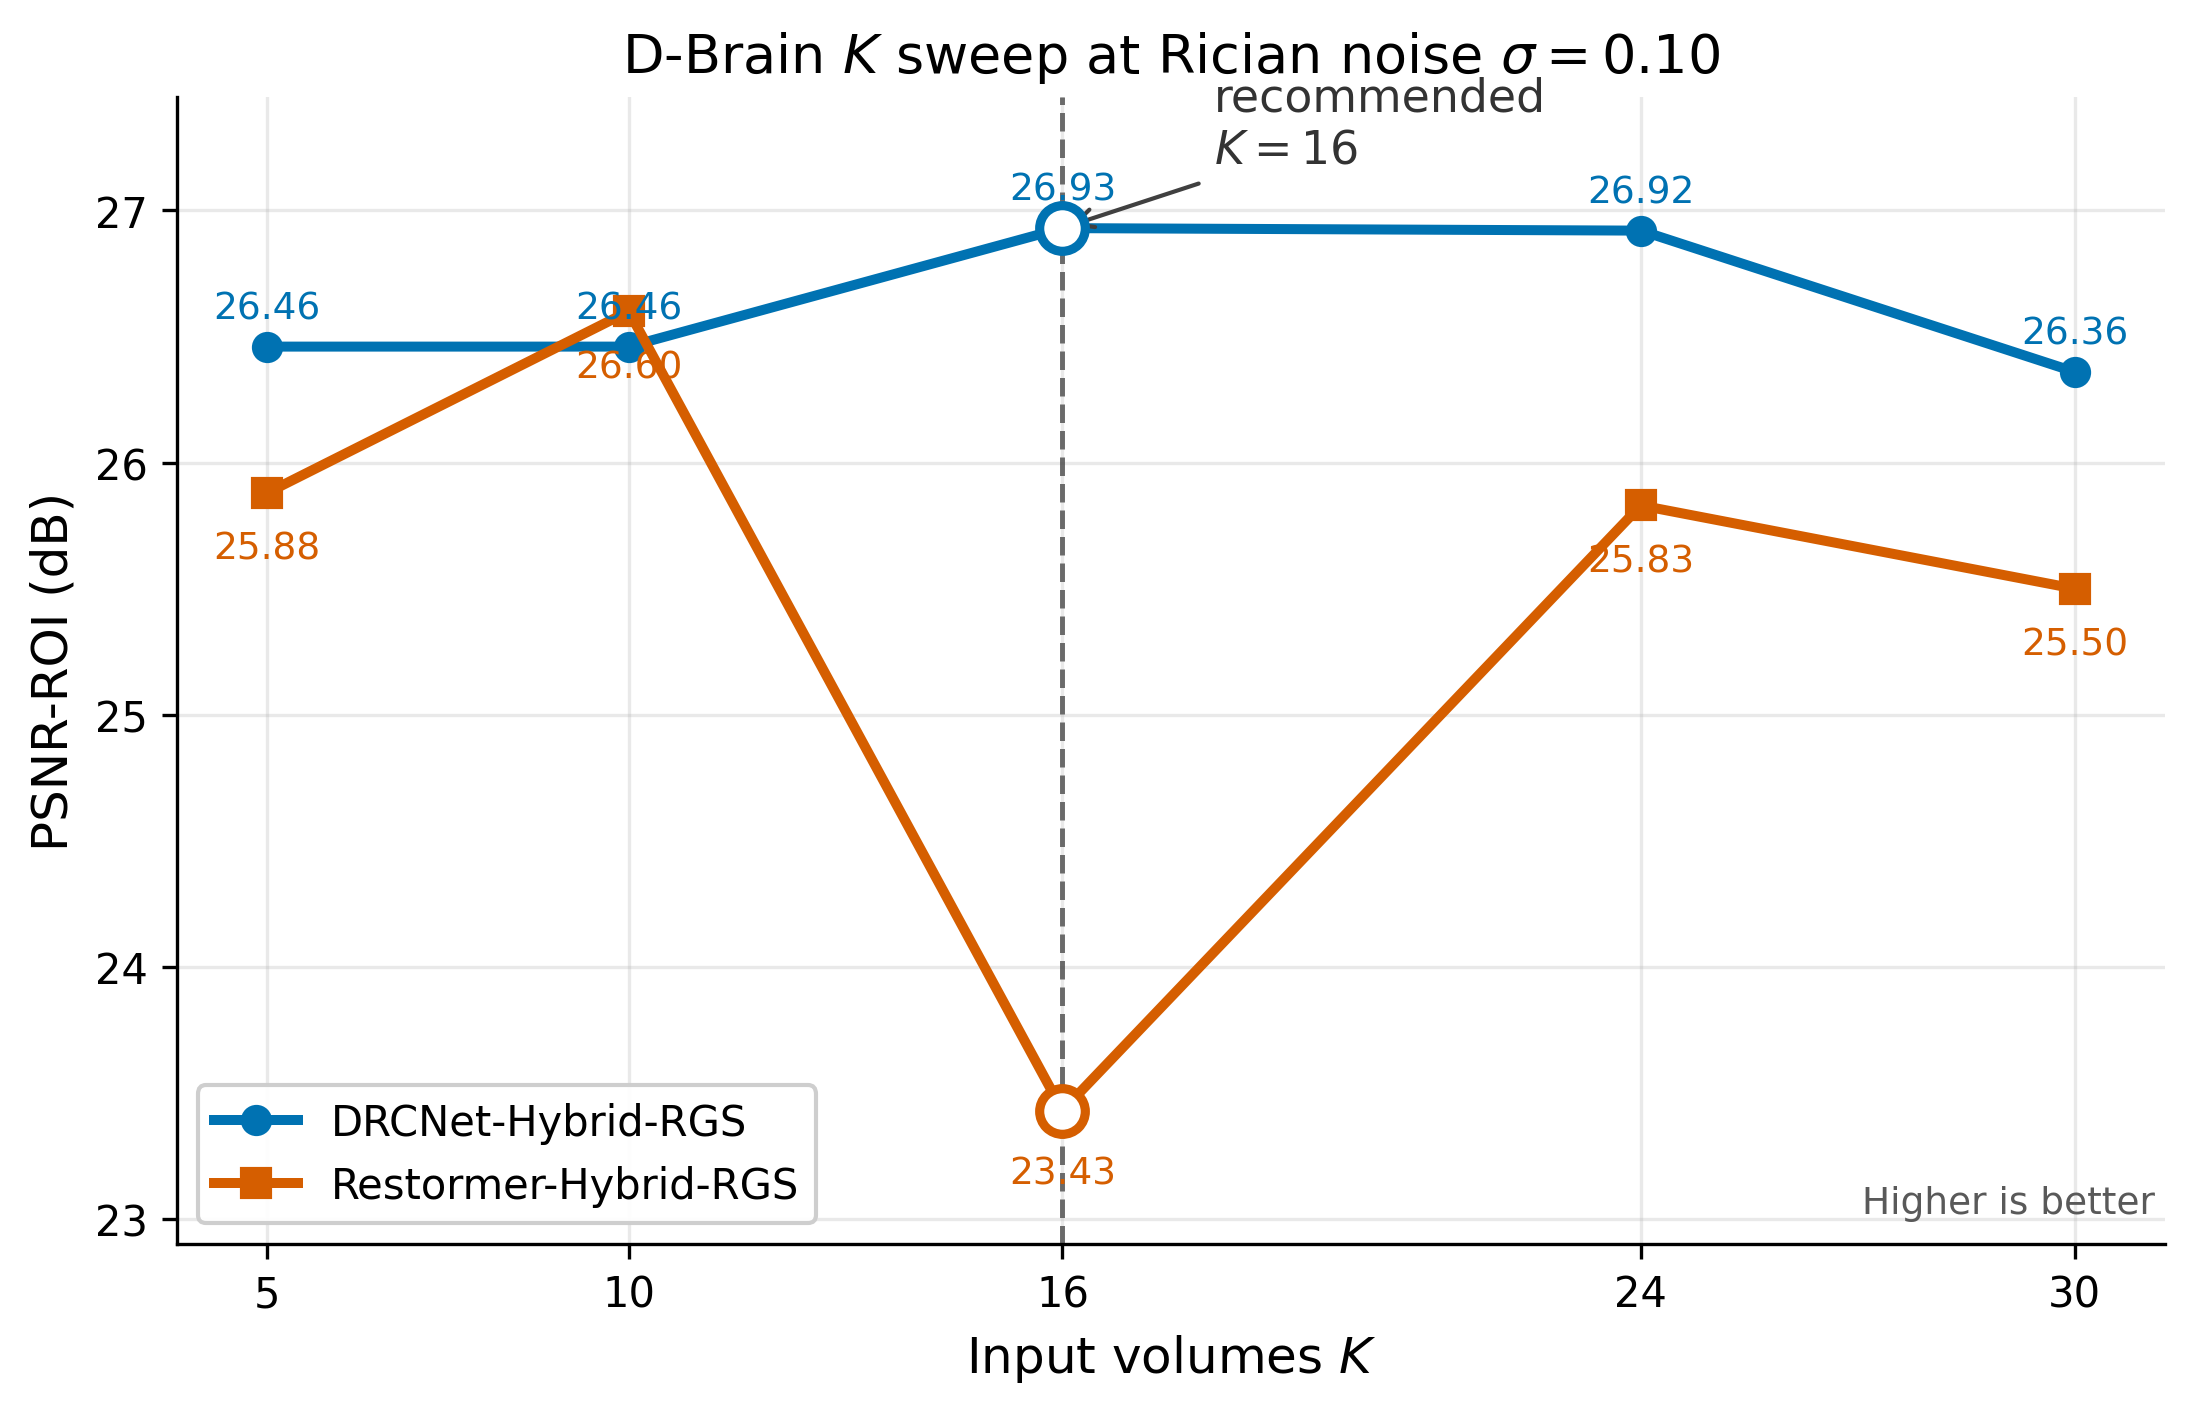
\includegraphics[width=0.78\linewidth]{figures/k_sweep_psnr_roi.png}
  \caption{$K$-sweep visualization on D-Brain. The plot shows PSNR-ROI versus $K \in \{5,10,16,24,30\}$ for DRCNet and Restormer, with the fixed cross-model operating point $K=16$ annotated.}
  \label{fig:k_sweep}
\end{figure}

Figure~\ref{fig:k_sweep} presents the same tradeoff as a quality-versus-input-size curve. Hybrid RGS does not require a large fraction of the diffusion volumes to be processed simultaneously: moderate subsets provide useful angular context while preserving feasible 3D training and inference. However, the optimal subset size remains backbone dependent.

\subsection{Backbone Capacity and Spatial Dimensionality}
\label{subsec:capacity_dimensionality}
A critical question for Hybrid RGS is whether its gains depend on volumetric neural processing or persist across different backbone choices. Many self-supervised denoising methods process medical images slice by slice using two-dimensional convolutions, whereas 3D models can exploit inter-slice anatomical continuity. This evaluation therefore has two components. First, Plain-CNN-2D and Res-CNN-2D test whether Hybrid RGS remains effective with independent, low-capacity slice-wise architectures. Second, the Restormer family provides controlled comparisons of spatial dimensionality and backbone capacity. Comparisons involving DRCNet3D, Plain-CNN-2D, and Res-CNN-2D are cross-architecture evaluations and should not be interpreted as matched 2D-versus-3D ablations.

All models in Table~\ref{tab:3d_vs_2d} use the fixed $K=16$ operating point, Bernoulli target masking, and the same core Hybrid RGS training protocol. The 3D models process volumetric D-Brain patches, whereas the 2D models process axial slices independently without explicit through-plane convolution or attention. Plain-CNN-2D and Res-CNN-2D are generic architectures implemented solely to test the sufficiency of lightweight 2D backbones. The controlled family comparison consists of Restormer-2D, baseline Restormer3D, and large Restormer3D. Restormer-2D follows the original two-dimensional formulation and is approximately capacity matched to baseline Restormer3D; large Restormer3D scales the same volumetric architecture to approximately $2.10$M parameters. Baseline and large Restormer3D share the sampling, masking, training, and evaluation settings described in Section~\ref{subsec:architectures}, so their differences are interpreted primarily as capacity effects.

The independent 2D results demonstrate that Hybrid RGS can achieve strong performance with inexpensive slice-wise architectures. Plain-CNN-2D obtains the highest PSNR-ROI in the table ($27.11$~dB), with SSIM-ROI $=0.5569$, FA-MAE $=0.2296$, and MD-MAE $=3435$. Res-CNN-2D reaches $26.44$~dB PSNR-ROI, $0.5504$ SSIM-ROI, $0.2309$ FA-MAE, and $3432$ MD-MAE. DRCNet3D achieves $26.93$~dB PSNR-ROI but uses substantially more parameters than either generic 2D model. These results establish backbone flexibility rather than a controlled dimensionality advantage. Cross-architecture rankings are also operating-point dependent: Restormer reaches $26.60$~dB PSNR-ROI at $K=10$, whereas Table~\ref{tab:3d_vs_2d} uses $K=16$.

Within the Restormer family, Restormer-2D outperforms baseline Restormer3D in PSNR-ROI ($25.25$ versus $23.43$~dB) and SSIM-ROI ($0.5840$ versus $0.5107$), and achieves a slightly lower FA-MAE ($0.2232$ versus $0.2238$). Baseline Restormer3D has a slightly lower MD-MAE ($3440$ versus $3447$). Restormer-2D also reduces inference time from $126.8$ to $26.7$~s per volume, a $4.7\times$ speedup. This approximately capacity-matched comparison indicates that the original two-dimensional Restormer formulation performs better than the volumetric extension on most reported metrics at this operating point. Restormer-2D also attains the lowest FA-MAE among all architectures in the table.

The large Restormer3D model provides the complementary capacity comparison. Increasing the volumetric model from $0.178$M to $2.10$M parameters raises PSNR-ROI by $2.51$~dB, from $23.43$ to $25.94$~dB, and produces the best SSIM-ROI ($0.5975$) and MD-MAE ($3422$) in the table. These gains indicate that capacity explains a substantial portion of the baseline Restormer3D image-domain deficit. However, FA-MAE worsens from $0.2238$ to $0.2596$, and inference time increases to $362.4$~s per volume, approximately $2.9\times$ the baseline Restormer3D cost and $13.6\times$ the Restormer-2D cost. The result remains specific to $K=16$.

Overall, the independent 2D models support the architecture-agnostic contribution of Hybrid RGS, while the Restormer comparisons isolate the effects of dimensionality and capacity. The results do not establish a uniform advantage for either 2D or 3D processing across all metrics. Qualitative inspection of reconstructed volumes, FA maps, and tractography-derived summaries remains necessary to determine whether higher-capacity volumetric models reduce through-plane discontinuities that are not strongly penalized by PSNR or voxelwise tensor errors.

The independent 2D architectures are also the least expensive: Plain-CNN-2D uses $0.014$M parameters and requires $4.7$~s per target volume, while Res-CNN-2D uses $0.015$M parameters and requires $3.9$~s. DRCNet3D requires $34.1$~s, but this cross-architecture difference is not a matched speedup. Within the Restormer family, Restormer-2D provides the controlled computational comparison described above, whereas large Restormer3D incurs the highest cost. Thus, higher-capacity volumetric processing improves selected image-domain metrics but requires substantially more computation and does not improve FA-MAE.

\begin{table}[ht]
  \centering
  \caption{Backbone capacity and spatial dimensionality evaluation on D-Brain with Rician noise $\sigma=0.1$ and $K=16$. All architectures use the same Hybrid RGS sampling and masked self-supervised loss. Plain-CNN-2D and Res-CNN-2D are independent lightweight architectures used to test whether Hybrid RGS performs effectively with generic slice-wise backbones; they are not ports of DRCNet or Restormer. Restormer-2D, baseline Restormer3D, and large Restormer3D form the controlled family comparison for spatial dimensionality and capacity. Bold marks the best overall value in each metric column.}
  \label{tab:3d_vs_2d}
  \resizebox{\linewidth}{!}{%
    \begin{tabular}{llcccccc}
      \toprule
      Backbone & Processing & PSNR-ROI $\uparrow$ & SSIM-ROI $\uparrow$ & FA-MAE $\downarrow$ & MD-MAE$^\dagger$ (a.u.) $\downarrow$ & Params (M) & Time/vol. (s) \\
      \midrule
      \multicolumn{8}{l}{\textit{Cross-architecture evaluations (not family matched)}} \\
      DRCNet3D & Volumetric & 26.93 & 0.5247 & 0.2575 & 3451 & 0.116 & 34.1 \\
      Plain-CNN-2D & Slice-wise & \textbf{27.11} & 0.5569 & 0.2296 & 3435 & \textbf{0.014} & 4.7 \\
      Res-CNN-2D & Slice-wise & 26.44 & 0.5504 & 0.2309 & 3432 & 0.015 & \textbf{3.9} \\
      \midrule
      \multicolumn{8}{l}{\textit{Restormer family (controlled comparisons)}} \\
      Restormer-2D & Slice-wise & 25.25 & 0.5840 & \textbf{0.2232} & 3447 & 0.149 & 26.7 \\
      Restormer3D & Volumetric & 23.43 & 0.5107 & 0.2238 & 3440 & 0.178 & 126.8 \\
      Restormer3D (large, $\approx2.10$M) & Volumetric & 25.94 & \textbf{0.5975} & 0.2596 & \textbf{3422} & 2.10 & 362.4 \\
      \bottomrule
    \end{tabular}
  }
\end{table}
\par\noindent\textit{Note:} $^\dagger$Diffusivity errors are in arbitrary D-Brain phantom units; compare across methods, not as physical mm$^2$/s values.

\subsection{Robustness to Noise Level}
The effective signal-to-noise ratio and artifact severity of DW-MRI data vary with scanner hardware, field strength, coil sensitivity, acquisition time, acceleration, and patient motion. A practical denoising method should therefore behave predictably across signal-to-noise regimes rather than being tuned to a single synthetic noise level. We assess this behavior by varying the Rician noise level on D-Brain and examining whether Hybrid RGS degrades gradually while preserving diffusion-derived quantities. This is a matched-noise experiment rather than a cross-noise transfer study: each model is trained and evaluated at the same noise level. The results therefore characterize the robustness of the training protocol across noise conditions, not generalization to an unseen noise distribution.

We evaluate $\sigma \in \{0.05,0.10,0.15,0.20\}$ using the same D-Brain ground-truth reference and the same Hybrid RGS configuration ($K=16$). DRCNet-Hybrid-RGS and Restormer-Hybrid-RGS are trained separately at each noise level, and MP-PCA is evaluated at all four levels. Patch2Self and MD-S2S results are available only for $\sigma=0.05$ and $0.10$. The analysis focuses on PSNR-ROI as the primary image-domain metric and FA-MAE as a downstream tensor-preservation metric. The $\sigma=0.10$, $K=16$ entries correspond to the primary experimental condition; models trained for other ablations are reported only in their respective ablation tables.

Table~\ref{tab:sigma_sweep} and Figure~\ref{fig:sigma_robustness} show an overall decline in PSNR-ROI as the noise level increases. MP-PCA achieves the highest PSNR-ROI at every tested level, from $33.33$ dB at $\sigma=0.05$ to $23.55$ dB at $\sigma=0.20$. Its strong performance is consistent with local PCA assumptions being well matched to spatially homogeneous synthetic Rician corruption. DRCNet-Hybrid-RGS declines from $29.76$ to $23.52$ dB across the sweep. Restormer-Hybrid-RGS declines from $27.19$ to $23.02$ dB overall, with a partial recovery at $\sigma=0.15$. Both neural models remain stable and show gradual degradation rather than abrupt failure.

The low-noise regime illustrates the tradeoff between classical denoising and learned self-supervision. At $\sigma=0.05$, MP-PCA achieves the best PSNR-ROI and FA-MAE. DRCNet-Hybrid-RGS nevertheless substantially outperforms Patch2Self ($29.76$ versus $23.74$ dB) and MD-S2S ($16.77$ dB) in image-domain fidelity. Restormer-Hybrid-RGS has lower PSNR-ROI than DRCNet but also a lower, better FA-MAE ($0.2170$ versus $0.2579$). Thus, the methods occupy different positions in the image-fidelity versus tensor-preservation tradeoff even under mild corruption.

At higher noise levels, DRCNet-Hybrid-RGS remains close to MP-PCA in PSNR-ROI: $25.11$ versus $25.54$ dB at $\sigma=0.15$ and $23.52$ versus $23.55$ dB at $\sigma=0.20$. However, MP-PCA retains substantially lower FA-MAE across all tested noise levels. Hybrid RGS is therefore robust in the sense of stable training and gradual degradation across matched noise conditions, but it does not uniformly surpass MP-PCA under this synthetic noise model. This result reinforces the need to report both image-domain fidelity and diffusion-derived errors rather than relying on PSNR alone.

\begin{table}[ht]
  \centering
  \caption{Noise-level robustness on D-Brain. Values are PSNR-ROI (dB); FA-MAE is shown in parentheses for the proposed methods and MP-PCA. Patch2Self and MD-S2S are available only at $\sigma=0.05$ and $0.10$. Each neural model is trained and evaluated at the same Rician noise level. Bold indicates the highest PSNR-ROI at each noise level.}
  \label{tab:sigma_sweep}
  \resizebox{\linewidth}{!}{%
    \begin{tabular}{lccccc}
      \toprule
      $\sigma$ & MP-PCA & Patch2Self & MD-S2S & DRCNet-Hybrid-RGS & Restormer-Hybrid-RGS \\
      \midrule
      0.05 & \textbf{33.33} (0.1009) & 23.74 & 16.77 & 29.76 (0.2579) & 27.19 (0.2170) \\
      0.10 & \textbf{28.44} (0.0898) & 21.31 & 15.28 & 26.93 (0.2575) & 23.43 (0.2238) \\
      0.15 & \textbf{25.54} (0.0978) & -- & -- & 25.11 (0.2202) & 24.63 (0.2452) \\
      0.20 & \textbf{23.55} (0.0863) & -- & -- & 23.52 (0.2211) & 23.02 (0.2597) \\
      \bottomrule
    \end{tabular}
  }
\end{table}

\begin{figure}[H]
  \centering
  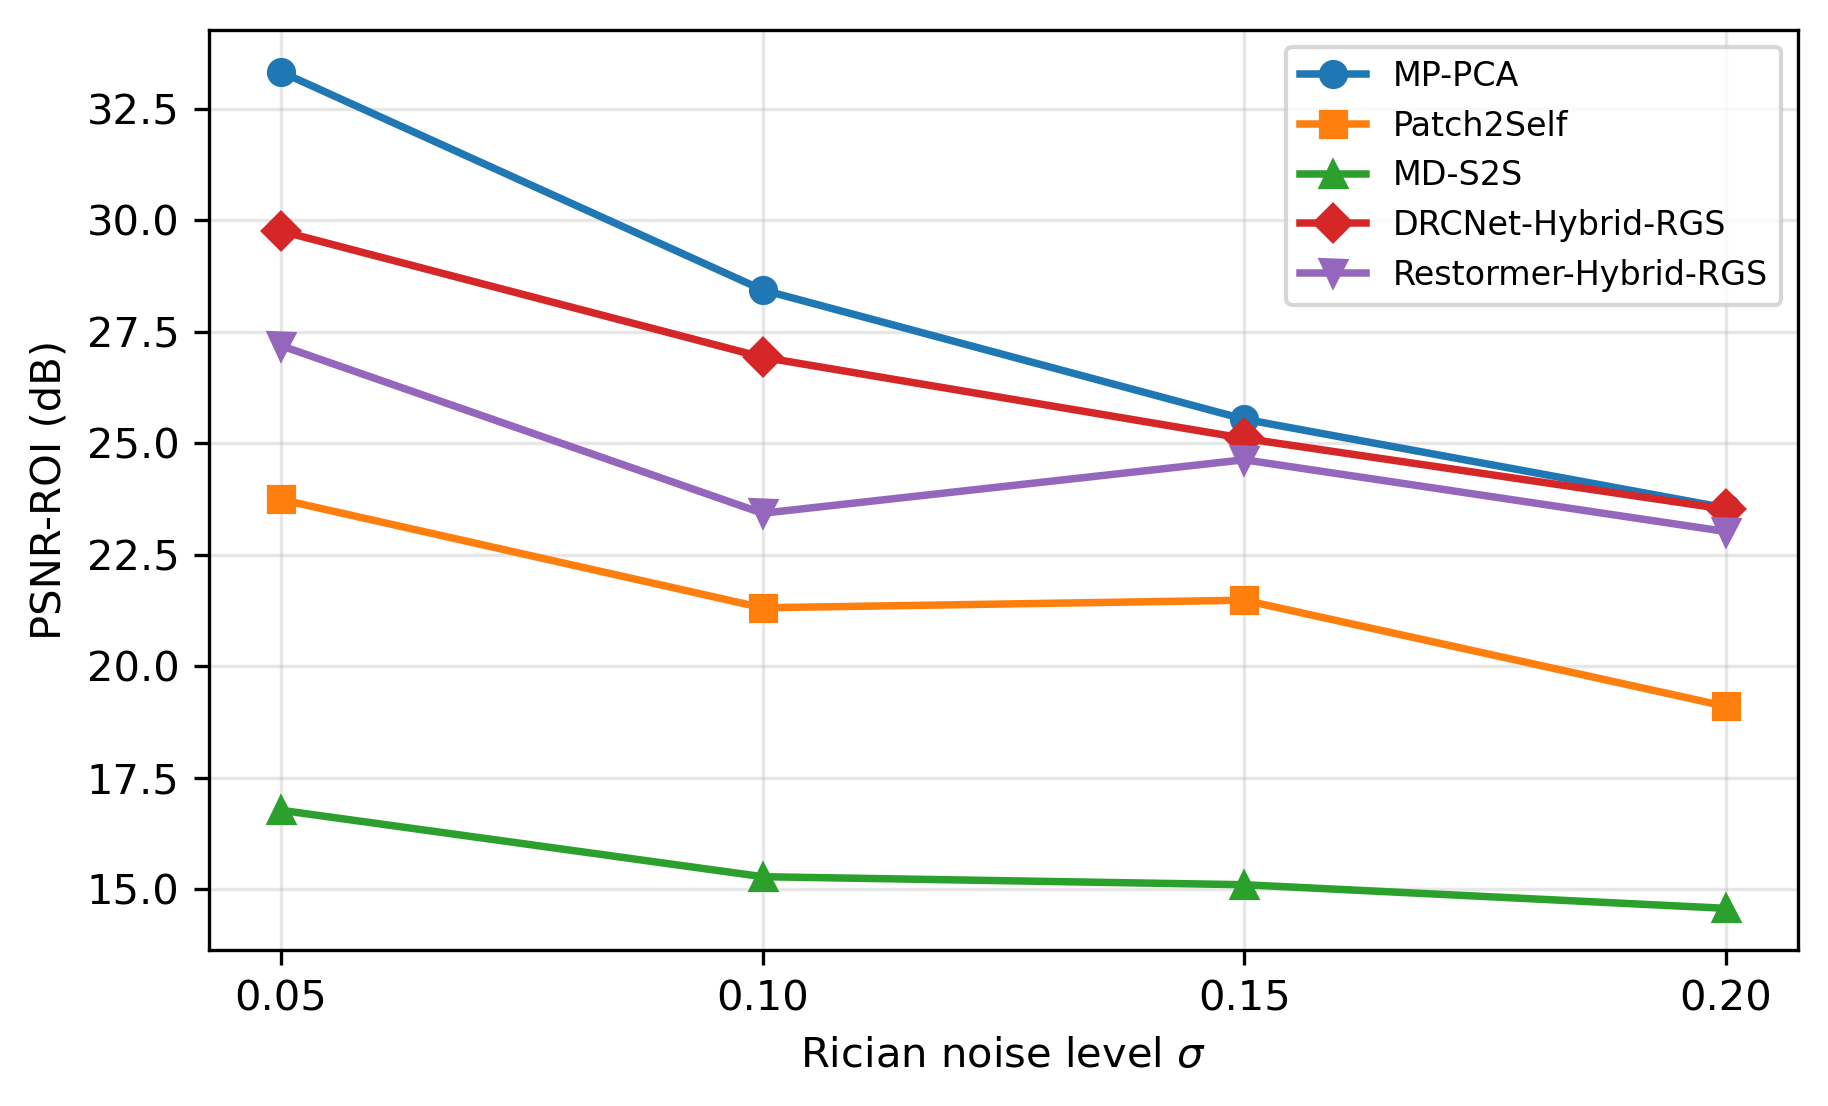
\includegraphics[width=0.78\linewidth]{figures/sigma_robustness_psnr_roi.png}
  \caption{Noise-robustness curve on D-Brain. The plot shows PSNR-ROI versus Rician noise level $\sigma \in \{0.05,0.10,0.15,0.20\}$. Patch2Self and MD-S2S are plotted only at $\sigma=0.05$ and $0.10$, where results are available.}
  \label{fig:sigma_robustness}
\end{figure}

\subsection{Gradient Direction Conditioning via FiLM}
\label{subsec:film_ablation}

In the baseline Hybrid RGS formulation, the $K$-channel input stack is randomly sampled and reordered at each training step. Although the target always occupies the final channel, the network receives no explicit information about its physical diffusion direction or $b$-value. We therefore investigate whether conditioning on target-gradient metadata can improve denoising in regions where the diffusion signal depends strongly on local fiber orientation. This mechanism is evaluated as an optional extension rather than a required component of Hybrid RGS.

We initially considered an additive input-level orientation encoding in which the metadata for each volume were projected into a learned spatial pattern and added to the input channels. This design was not evaluated because it converts spatially invariant acquisition metadata into an artificial image-like signal, conditions every context channel, and may be diluted as features propagate through the network. These limitations motivated target-specific conditioning in feature space.

We instead use Feature-wise Linear Modulation (FiLM) \cite{perez2018film} as a lightweight feature-space conditioning mechanism. Given an intermediate feature tensor $F$ at layer $\ell$, FiLM applies
\begin{equation}
  \operatorname{FiLM}_\ell(F) = \gamma_\ell(q_t) \odot F + \beta_\ell(q_t),
  \label{eq:film}
\end{equation}
where the channel-wise scale $\gamma_\ell(q_t)$ and shift $\beta_\ell(q_t)$ are predicted by a small multilayer perceptron from the target condition vector $q_t=[\cos_x,\cos_y,\cos_z,b_{\mathrm{norm}}]$. The modulation parameters are broadcast across spatial locations. Because $q_t$ describes only the target volume, the model is informed about the direction it must reconstruct without separately conditioning the randomly sampled context volumes.

FiLM preserves the spatial invariance of the acquisition metadata while allowing conditioning at multiple feature depths. The FiLM layers use identity initialization, with $\gamma_\ell$ initialized near one and $\beta_\ell$ near zero, so the conditioned networks begin close to their unconditioned baselines.

In DRCNet-Hybrid-RGS, FiLM is inserted at two feature stages of the 3D convolutional backbone. In Restormer-Hybrid-RGS, it is inserted at three stages of the transformer-style restoration hierarchy. The parameter overhead is approximately $3.4\%$ for DRCNet and $3.9\%$ for Restormer, based on the rounded parameter counts in Table~\ref{tab:film_ablation}. The conditioning does not weaken the blind-spot construction because the metadata are deterministic acquisition descriptors and do not reveal the noisy voxel intensities evaluated by the masked loss.

\begin{table}[ht]
  \centering
  \caption{Gradient direction conditioning ablation on D-Brain. FiLM improves full-volume PSNR for both backbones but slightly degrades PSNR-ROI, indicating metric-dependent behavior rather than a uniform denoising benefit.}
  \label{tab:film_ablation}
  \resizebox{\linewidth}{!}{%
    \begin{tabular}{llcccccc}
      \toprule
      Model & Conditioning & PSNR (dB) $\uparrow$ & PSNR-ROI (dB) $\uparrow$ & FA-MAE $\downarrow$ & MD-MAE$^\dagger$ (a.u.) $\downarrow$ & Params & Time/vol. \\
      \midrule
      DRCNet & Baseline RGS & 23.90 & 26.93 & 0.2575 & 3451 & 116K & 34.1 s \\
      DRCNet & FiLM & 25.40 & 26.24 & 0.2405 & 3452 & 120K & 35.3 s \\
      DRCNet & $\Delta$ FiLM $-$ baseline & +1.50 & $-0.69$ & $-6.6\%$ & +0.0\% & +3.4\% & +3.5\% \\
      \midrule
      Restormer & Baseline RGS & 22.98 & 23.43 & 0.2238 & 3440 & 178K & 126.8 s \\
      Restormer & FiLM & 23.60 & 22.69 & 0.2603 & 3423 & 185K & 130.3 s \\
      Restormer & $\Delta$ FiLM $-$ baseline & +0.62 & $-0.74$ & +16.3\% & $-0.5\%$ & +3.9\% & +2.8\% \\
      \bottomrule
    \end{tabular}
  }
\end{table}
\par\noindent\textit{Note:} $^\dagger$Diffusivity errors are in arbitrary D-Brain phantom units; compare across methods, not as physical mm$^2$/s values.

As summarized in Table~\ref{tab:film_ablation}, FiLM has mixed effects on D-Brain. For DRCNet, conditioning increases full-volume PSNR from $23.90$ to $25.40$ dB, a gain of $1.50$ dB, but decreases PSNR-ROI from $26.93$ to $26.24$ dB. Thus, the full-volume improvement is not reflected within the brain-tissue ROI. FA-MAE improves by $6.6\%$, while MD-MAE changes by only one unit, from $3451$ to $3452$.

For Restormer, FiLM increases full-volume PSNR by $0.62$ dB but decreases PSNR-ROI from $23.43$ to $22.69$ dB. MD-MAE improves slightly, from $3440$ to $3423$, whereas FA-MAE worsens by $16.3\%$. Again, the full-volume gain does not translate into consistent improvement within the brain ROI or across tensor-derived metrics. FiLM should therefore be interpreted as an exploratory mechanism that requires architecture-specific tuning rather than as a recommended default.

The effect of FiLM is therefore both metric and backbone dependent. DRCNet shows a larger full-volume PSNR gain and improved FA-MAE, whereas Restormer shows a smaller PSNR gain and worsened FA-MAE. Both backbones lose PSNR-ROI, suggesting that FiLM placement, initialization, regularization, or tensor-aware model selection requires further study before conditioning can be claimed to improve anatomically relevant regions. FiLM-conditioned models can also be trained on Stanford HARDI with $G=150$ gradients and $b=2000~\mathrm{s/mm^2}$; however, no matching unconditioned Stanford run is available under the same evaluation protocol. The Stanford experiments therefore establish feasibility only and are not used to claim a quantitative conditioning benefit.

\subsection{Implementation Details}
\paragraph{Training}\mbox{}\\
All neural models are trained with Adam using a base learning rate of $4.5 \times 10^{-4}$ and no learning-rate schedule. Automatic mixed precision (AMP) is enabled to reduce GPU memory consumption. Random seeds 91021 and 91022 are used for the D-Brain and Stanford experiments, respectively. Deterministic settings are enabled for PyTorch, NumPy, and the Hybrid RGS gradient sampler. At each progressive D-Brain stage, $60\%$ of the extracted patches are retained through seeded random subsampling. Exact bitwise agreement across hardware and software environments is not guaranteed.

\paragraph{Progressive schedule}\mbox{}\\
The primary DRCNet3D and Restormer3D models use the same three-stage progressive patch protocol (Table~\ref{tab:implementation_schedule}), with architecture-specific batch sizes selected to fit GPU memory. At the beginning of each stage, patches are re-extracted at the specified resolution and the Adam optimizer is re-initialized at the same base learning rate; model weights are retained from the preceding stage. D-Brain uses 120 epochs per stage (360 epochs total), whereas Stanford HARDI uses 300 epochs per stage (900 epochs total). The 2D architectures use the corresponding in-plane patch sizes and strides with architecture-specific batch sizes.

\begin{table}[t]
  \centering
  \caption{Progressive training schedule for the primary DRCNet3D and Restormer3D models. Patch sizes are cubic for the 3D models; the 2D architectures use the corresponding in-plane sizes and strides.}
  \label{tab:implementation_schedule}
  \resizebox{\linewidth}{!}{%
    \begin{tabular}{lcccccc}
      \toprule
      Stage & Patch size & Stride & Batch size (DRCNet3D) & Batch size (Restormer3D) & D-Brain epochs & Stanford epochs \\
      \midrule
      1 & $32^3$ voxels & 8 & 128 & 64 & 120 & 300 \\
      2 & $24^3$ voxels & 6 & 256 & 128 & 120 & 300 \\
      3 & $16^3$ voxels & 4 & 256 & 256 & 120 & 300 \\
      \bottomrule
    \end{tabular}
  }
\end{table}

\paragraph{Augmentation}\mbox{}\\
No explicit geometric augmentation, such as flips, rotations, or elastic deformations, is applied. Training stochasticity instead arises from random gradient-subset sampling, independent Bernoulli masks for each sample, and strided patch extraction across spatial locations. For D-Brain, patches satisfying $\max(x_{\mathrm{patch}}) \leq 0.02$ on the clean phantom are discarded to exclude near-zero padding regions. The clean reference is used only for this background-filtering step and does not serve as a training target or enter checkpoint selection. No patch filtering is applied to Stanford HARDI.

\paragraph{Normalization}\mbox{}\\
Each diffusion-weighted volume is independently min--max normalized to $[0,1]$ before training. Denoised outputs are clipped to this range for image-domain evaluation. Before tensor fitting, the stored per-volume minimum and maximum values are used to restore the outputs to the original phantom intensity scale.

\paragraph{Inference}\mbox{}\\
Full-volume reconstruction uses Monte Carlo averaging over random context subsets and target masks. D-Brain evaluation uses $N_c=16$ context samples and $N_p=12$ mask draws per context, whereas Stanford HARDI uses $N_c=16$ and $N_p=23$. Predictions are processed in chunks of four to control GPU memory. The volumetric Restormer models additionally use overlapping tiled inference with Gaussian weighting, a patch size of 32 voxels, and a one-voxel overlap.

\paragraph{Hardware and timing}\mbox{}\\
All experiments are performed on a single NVIDIA Tesla T4 GPU with 15~GB of VRAM, CUDA~12.2, and PyTorch~2.x. A complete 360-epoch D-Brain training run requires approximately 8--12 hours, depending on the backbone. Across the architectures in Table~\ref{tab:3d_vs_2d}, inference time per target diffusion volume ranges from $3.9$~s for Res-CNN-2D to $362.4$~s for large Restormer3D.

\paragraph{Checkpoint selection}\mbox{}\\
For evaluation, the final-stage checkpoint with the lowest epoch-averaged self-supervised training loss is retained. Validation-set early stopping is not used because clean validation targets are unavailable. Exact bitwise agreement across GPU types and software environments is not expected.

\section{Experimental Results}
\subsection{Main Comparison}
Table~\ref{tab:main_comparison} summarizes the primary quantitative evaluation on the D-Brain dataset with synthetic Rician noise at $\sigma=0.1$. Hybrid RGS methods use $K=16$ input gradient volumes as a fixed operating point for cross-model comparability. Because D-Brain contains $G=60$ diffusion-weighted directions, each Hybrid RGS sample uses only 15 non-target context gradients and one masked target, rather than the 59 non-target predictors used by leave-one-volume-out Patch2Self. This shared setting favors DRCNet: as shown in Table~\ref{tab:sampling_ablations}, DRCNet peaks at $K=16$ ($26.93$~dB PSNR-ROI), whereas Restormer's strongest result in the $K$ sweep occurs at $K=10$ (PSNR-ROI $=26.60$~dB, FA-MAE $=0.2195$). The Restormer row in the main comparison therefore represents the fixed cross-model operating point rather than its best configuration from the sweep. The table compares the proposed self-supervised 3D models with the classical and self-supervised baselines MP-PCA \cite{veraart2016mppca}, Patch2Self with the DIPY OLS backend \cite{fadnavis2020patch2self}, and MD-S2S with a two-dimensional convolutional masking strategy \cite{kang2024mds2s}. Supervised DRCNet and Restormer variants are included as reference runs to contextualize the self-supervised results; they are not intended as rigorously tuned upper bounds.

MP-PCA remains a strong classical preprocessing baseline. It achieves $28.44$~dB PSNR-ROI and the lowest FA-MAE in this experiment ($0.0898$), suggesting that its local PCA assumptions preserve tensor anisotropy well under the tested synthetic noise model. However, its MD-MAE remains high ($4650$), showing that improved FA preservation does not necessarily imply uniform improvement across diffusion-tensor scalar measures. Patch2Self provides a self-supervised angular baseline using leave-one-volume-out OLS regression. Its PSNR-ROI is lower ($21.31$~dB), but its MD-MAE ($3438$) is competitive with those of the neural self-supervised methods, consistent with the angular redundancy of DWI. Among the non-Hybrid self-supervised baselines, MD-S2S obtains the lowest FA-MAE ($0.2298$) but the lowest image-domain fidelity, with $15.28$~dB PSNR-ROI. Because this comparison changes the method, architecture, and training objective simultaneously, the lower image-domain performance cannot be attributed to slice-wise processing alone.

The proposed Hybrid RGS models combine the angular self-supervision of Patch2Self with the blind-spot spatial masking of Self2Self-style methods. DRCNet-Hybrid-RGS achieves the strongest self-supervised image-domain results in the table: $23.90$~dB PSNR, $0.4402$ SSIM, and $26.93$~dB PSNR-ROI. Relative to Patch2Self, this corresponds to a $5.62$~dB gain in PSNR-ROI and an approximately $73\%$ reduction in ROI MSE, based on the rounded table values. Relative to MD-S2S, DRCNet-Hybrid-RGS improves PSNR-ROI by $11.65$~dB, consistent with the benefit of coupling random angular context with target-channel masking. Its FA-MAE ($0.2575$) is slightly higher than those of Patch2Self and MD-S2S, whereas its MD-MAE ($3451$) remains close to the best self-supervised values.

Restormer-Hybrid-RGS obtains lower full-volume PSNR ($22.98$~dB) and ROI PSNR ($23.43$~dB) than DRCNet at the fixed $K=16$ operating point. Its FA-MAE ($0.2238$) is lower than DRCNet's ($0.2575$), while its MD-MAE ($3440$) is close to that of Patch2Self. Importantly, this comparison does not reflect Restormer's best configuration from the sweep: Table~\ref{tab:sampling_ablations} shows Restormer peaking at $K=10$ with PSNR-ROI $=26.60$~dB and FA-MAE $=0.2195$. Compared with DRCNet at $K=16$, this result is competitive in PSNR-ROI and better in FA-MAE, although the two values come from different operating points. The gap in the main table is therefore partly associated with the shared $K=16$ setting rather than necessarily reflecting an inherent limitation of the Restormer backbone. DRCNet is also substantially faster at $K=16$, requiring $34.1$~s per target volume compared with $126.8$~s for Restormer. Thus, the main comparison supports DRCNet-Hybrid-RGS as the more practical instantiation at this fixed operating point, while Restormer provides a complementary test of backbone sensitivity.

The supervised reference runs provide context for interpreting the self-supervised results and are not intended as rigorously tuned upper bounds. They use the corresponding DRCNet and Restormer backbones with the same input-sampling and optimization settings: $K=16$, RGS gradient sampling, random seed 91021, $60\%$ random patch subsampling, Adam at $4.5\times10^{-4}$, checkpoint selection based on the lowest training loss, and the same single-subject D-Brain setting. The supervised models retain the noisy RGS inputs but are optimized against clean D-Brain phantom targets rather than masked noisy target voxels. Supervised DRCNet reaches $22.92$~dB PSNR-ROI, while supervised Restormer reaches $22.60$~dB. In the present runs, these supervised reference models do not exceed DRCNet-Hybrid-RGS in image-domain metrics. This outcome should not be generalized as evidence that supervision is intrinsically inferior to self-supervision: the single-subject, limited-data setting, Rician noise structure, and absence of comparably tuned supervised hyperparameters may all contribute. The more important observation is that Hybrid RGS achieves competitive performance without clean training targets, which is valuable in clinical and research DWI settings where paired noisy--clean acquisitions are unavailable or prohibitively expensive.

\begin{table}[ht]
  \centering
  \caption{Main quantitative comparison on D-Brain with Rician noise $\sigma=0.1$. All Hybrid RGS methods use the fixed $K=16$ cross-model operating point. ROI metrics are computed over brain tissue only ($\Omega_{\mathrm{ROI}}^{\mathrm{eval}}$). Time/vol.\ is the inference time per target diffusion volume when available. Bold values indicate the best result among the self-supervised neural or regression rows in each metric column. Italicized rows are supervised reference runs that use the corresponding backbone, input-sampling protocol, and optimization settings with clean phantom targets; they are not rigorously tuned upper bounds.}
  \label{tab:main_comparison}
  \resizebox{\linewidth}{!}{%
    \begin{tabular}{lcccccccc}
      \toprule
      Method & PSNR $\uparrow$ & SSIM $\uparrow$ & MSE $\downarrow$ & PSNR-ROI $\uparrow$ & MSE-ROI $\downarrow$ & FA-MAE $\downarrow$ & MD-MAE$^\dagger$ (a.u.) $\downarrow$ & Time/vol. (s) \\
      \midrule
      MP-PCA & 22.59 & 0.4350 & 0.00551 & 28.44 & 0.00143 & 0.0898 & 4650 & -- \\
      Patch2Self (DIPY OLS) & 17.65 & 0.3806 & 0.01719 & 21.31 & 0.00739 & 0.2393 & \textbf{3438} & -- \\
      MD-S2S (Conv2D) & 15.14 & 0.4250 & 0.03061 & 15.28 & 0.02963 & 0.2298 & 3449 & -- \\
      DRCNet-Hybrid-RGS & \textbf{23.90} & \textbf{0.4402} & \textbf{0.00408} & \textbf{26.93} & \textbf{0.00203} & 0.2575 & 3451 & \textbf{34.1} \\
      Restormer-Hybrid-RGS & 22.98 & 0.4288 & 0.00504 & 23.43 & 0.00454 & \textbf{0.2238} & 3440 & 126.8 \\
      \midrule
      \textit{DRCNet supervised} & \textit{21.37} & \textit{0.3686} & \textit{0.00729} & \textit{22.92} & \textit{0.00511} & \textit{0.2387} & \textit{3684} & \textit{34.0} \\
      \textit{Restormer supervised} & \textit{21.57} & \textit{0.3696} & \textit{0.00697} & \textit{22.60} & \textit{0.00549} & \textit{0.2374} & \textit{3713} & \textit{125.3} \\
      \bottomrule
    \end{tabular}
  }
\end{table}
\par\noindent\textit{Note:} $^\dagger$MD-MAE for D-Brain rows is reported in arbitrary units derived from the phantom intensity scale and should be interpreted as a relative comparison across methods, not as a physical diffusivity in mm$^2$/s.

\todo[author=FHS,color=yellow, inline]{Replace this planned qualitative comparison with final image panels or remove the figure before submission. The final figure should include noisy input, MP-PCA, Patch2Self, MD-S2S, DRCNet-Hybrid-RGS, Restormer-Hybrid-RGS, reference image when available, and error maps.}

\subsection{Generalization to Real Scanner Noise}
The D-Brain experiments provide controlled quantitative evaluation because synthetic Rician noise is added to data with an available reference. However, this setting cannot fully represent real scanner noise, which may include thermal noise, Gibbs ringing, eddy-current residuals, motion, coil-dependent spatial variation, and deviations from an ideal Rician model in low-SNR regions. We therefore evaluate Hybrid RGS on Stanford HARDI as a complementary real-data experiment. Stanford HARDI uses a different acquisition protocol from D-Brain, with $b=2000~\mathrm{s/mm^2}$ and $G=150$ diffusion directions, compared with $b=2500~\mathrm{s/mm^2}$ and $G=60$ in the primary synthetic experiments. Because only a single acquisition is available, no clean ground truth exists; this section therefore emphasizes qualitative assessment, downstream FA/MD map plausibility, and scalability rather than PSNR/SSIM against a reference.

The Stanford experiment trains the same self-supervised models directly on the noisy Stanford data. We use the same Hybrid RGS objective with $K=16$, target-channel Bernoulli masking, and the same reconstruction loss; no clean targets are used. Although Stanford HARDI contains $G=150$ diffusion directions, each network input still contains only 15 randomly sampled context gradients and one masked target rather than scaling to 149 non-target channels. Patch2Self and MD-S2S are included as self-supervised baselines that are applicable without ground truth. MP-PCA can also be evaluated as a classical preprocessing method when available, but the central comparison is qualitative because all methods operate without an external reference. Evaluation focuses on visual inspection of denoised diffusion-weighted volumes, smoothness and anatomical plausibility of FA and MD maps, and reference-free stability measures such as variance within homogeneous tissue regions.

The Hybrid RGS models were successfully trained and applied to Stanford HARDI volumes. The method can be trained directly on real scanner data using the same self-supervised objective, and denoised outputs can be used to compute downstream tensor-derived maps. Visual assessment of denoised volumes and FA/MD maps requires the panels described in the TODO below; without those panels, Stanford results support feasibility and scalability rather than specific visual quality claims. FiLM-conditioned Stanford models yield internal-reference FA deviations of $0.0356$ for DRCNet-FiLM and $0.0756$ for Restormer-FiLM (deviation from the tensor fit of the acquired noisy signal, not ground-truth error); these numbers indicate that the pipeline can produce stable diffusion-derived summaries on real scanner data.

\todo[author=FHS,color=yellow, inline]{Add visual Stanford FA/MD panels, residual maps, and/or homogeneous-ROI variance summaries. Without those panels, keep Stanford claims limited to feasibility and scalability.}

Table~\ref{tab:stanford_k_sweep} summarizes the Stanford $K$ sweep using noisy-input PSNR-ROI, where the acquired noisy image is used as the comparison image. These values should not be compared with D-Brain PSNR and should not be interpreted as restoration accuracy; they measure closeness to the acquired signal. A method that changes the image very little can score well under this metric. For DRCNet, the noisy-input score increases from $34.86$ dB at $K=5$ to $39.47$ dB at $K=24$, then drops at $K=30$, suggesting that very large input stacks are not necessarily beneficial. Restormer increases from $23.79$ dB at $K=5$ to $27.08$ dB at $K=30$, but remains more computationally expensive. Inference time scales moderately with $K$ for DRCNet, from $23.5$ to $28.0$ s per volume, and remains around $84$--$85$ s for Restormer. Because noisy-input PSNR rewards input closeness rather than restoration accuracy, it should not be used to select $K$. Given the absence of ground truth, the Stanford sweep serves as a feasibility and runtime probe only. $K=16$ is retained as the cross-model operating point for consistency and cost, while $K=24$ or $K=30$ require validation with reference-free or test--retest criteria before recommendation.

FiLM conditioning also transfers to Stanford without architectural changes. The FiLM-conditioned DRCNet run achieves a noisy-input PSNR-ROI of $36.55$ dB with an inference time of $26.8$ s per volume, while the FiLM-conditioned Restormer run achieves $24.00$ dB with $85.4$ s per volume. These values measure input closeness rather than denoising accuracy. Their main value is that target-direction metadata can be incorporated in a real, larger-shell protocol without breaking the self-supervised training pipeline.

\begin{table}[ht]
  \centering
  \caption{Stanford HARDI $K$ sweep. PSNR-ROI is computed against the acquired noisy image and should be interpreted only as an input-closeness or signal-preservation measure rather than ground-truth restoration accuracy. Time/vol. is inference time per target diffusion volume.}
  \label{tab:stanford_k_sweep}
  \resizebox{\linewidth}{!}{%
    \begin{tabular}{llccc}
      \toprule
      Architecture & $K$ & Noisy-input PSNR-ROI & Params (M) & Time/vol. (s) \\
      \midrule
      DRCNet & 5 & 34.86 & 0.106 & 23.5 \\
      DRCNet & 10 & 36.99 & 0.111 & 25.3 \\
      DRCNet & 16 & 38.07 & 0.116 & 25.2 \\
      DRCNet & 24 & 39.47 & 0.123 & 26.3 \\
      DRCNet & 30 & 35.18 & 0.128 & 28.0 \\
      Restormer & 5 & 23.79 & 0.174 & 83.7 \\
      Restormer & 10 & 26.60 & 0.176 & 84.4 \\
      Restormer & 16 & 26.05 & 0.178 & 83.1 \\
      Restormer & 24 & 25.65 & 0.180 & 84.7 \\
      Restormer & 30 & 27.08 & 0.182 & 85.1 \\
      \bottomrule
    \end{tabular}
  }
\end{table}

\todo[author=FHS,color=yellow, inline]{Replace the planned Stanford HARDI FA-map comparison with final image panels or remove the figure before submission. The final figure should show a representative axial slice crossing major white-matter tracts for noisy input, Patch2Self, MD-S2S, DRCNet-Hybrid-RGS, and Restormer-Hybrid-RGS.}

Overall, the Stanford experiment supports the feasibility of Hybrid RGS beyond synthetic D-Brain corruption. The method can be trained directly on real scanner data, scales from $G=60$ to $G=150$ without architectural changes, and produces outputs suitable for qualitative FA/MD assessment. The main limitation is the absence of ground truth, which prevents claims of quantitative restoration accuracy. Future work should evaluate the same protocol on repeated acquisitions or test--retest datasets where one scan can serve as an approximate reference.

\section{Discussion}
The experiments support Hybrid RGS primarily as a reduced-angular-context self-supervised framework rather than as evidence for a single dominant architecture. Its central objective is to maintain effective denoising while limiting each sample to one masked target and $K-1$ randomly selected context gradients, rather than requiring all available directions simultaneously. Random subsets outperform sequential windows in ROI PSNR, indicating that changing the limited angular context across iterations provides useful diversity. Moderate input sizes can provide a practical compromise between denoising context, channel count, and computational cost, although the optimal $K$ is backbone dependent. FiLM conditioning is a promising but exploratory extension because deterministic acquisition metadata can be incorporated without weakening the blind-spot construction, but the present results show full-volume PSNR gains alongside ROI degradation. These findings identify the core contribution as coupling limited random angular context with target-channel masking, allowing DW-MRI denoisers to be trained without clean targets and instantiated with different backbones.

The architecture evaluation has two distinct components. First, the independent Plain-CNN-2D and Res-CNN-2D experiments show that Hybrid RGS can achieve strong performance with inexpensive slice-wise architectures. Because these models are not 2D versions of DRCNet or Restormer, their comparisons with the volumetric models jointly change architecture, capacity, and dimensionality and should not be interpreted as controlled 2D-versus-3D tests. Second, the Restormer family provides the controlled analysis: the original Restormer-2D formulation outperforms baseline Restormer3D in PSNR-ROI, SSIM-ROI, and FA-MAE at approximately matched capacity, whereas large Restormer3D recovers much of the image-domain deficit and achieves the best SSIM-ROI and MD-MAE at substantially greater computational cost and with worse FA-MAE. These findings show that the Hybrid RGS objective transfers across backbones, while conclusions about spatial dimensionality and capacity must be drawn from the Restormer family and remain specific to the selected operating point. The $K$ sweep reinforces this qualification because Restormer peaks at $K=10$, whereas the cross-architecture table uses $K=16$.

MP-PCA remains a strong baseline, particularly for FA preservation under synthetic Rician noise. This is expected because local low-rank assumptions are well matched to spatially homogeneous simulated corruption. The proposed neural models improve substantially over Patch2Self and MD-S2S in image-domain ROI metrics, but they do not uniformly dominate every diffusion-derived metric. Reporting both image fidelity and tensor-derived errors is therefore essential: improvements in PSNR or MSE do not necessarily imply better FA, MD, AD, or RD estimates.

The framework has several limitations. First, the self-supervised objective relies on independence assumptions about noise across masked dimensions and diffusion volumes; correlated motion, Gibbs ringing, or reconstruction artifacts may violate these assumptions. Second, synthetic Rician experiments cannot fully represent real scanner noise, and Stanford HARDI lacks ground truth, so its results support feasibility rather than quantitative accuracy. Third, high-capacity networks and conditioning mechanisms may introduce anatomically plausible but quantitatively biased signal if validation is based only on image-domain similarity. Future work should therefore treat architecture choice as an empirical design variable and emphasize repeated acquisitions, test--retest datasets, tractography endpoints, and reader studies to determine when Hybrid RGS improves clinically relevant diffusion analysis.

\section{Conclusion}
This manuscript presented Hybrid RGS, an architecture-agnostic self-supervised framework designed to denoise DW-MRI using small random gradient subsets and voxel-wise target masking. By fixing $K\ll G$, the method limits the number of gradients processed per training and inference sample while retaining access to the full acquisition through repeated random sampling. The results indicate that this strategy improves over Patch2Self and MD-S2S in image-domain ROI metrics on D-Brain, benefits from random rather than sequential angular sampling, and remains stable across synthetic Rician noise levels. The experiments also show that MP-PCA is a highly competitive baseline for FA preservation under synthetic noise, emphasizing the need to evaluate both image-domain and diffusion-domain metrics. Independent Plain-CNN-2D and Res-CNN-2D experiments demonstrate that Hybrid RGS can work effectively with lightweight slice-wise architectures; these models are not family-matched counterparts of DRCNet or Restormer. Within the controlled Restormer comparison at $K=16$, the original Restormer-2D formulation outperforms baseline Restormer3D on most reported metrics, while increasing Restormer3D capacity closes much of the image-domain gap at substantially greater computational cost and with worse FA-MAE. Conclusions about dimensionality and capacity are therefore based on the Restormer family and remain operating-point dependent, particularly because Restormer reaches its best $K$-sweep result at $K=10$. FiLM conditioning remains a lightweight but exploratory extension because it improves full-volume PSNR while degrading ROI PSNR in the present results, and Stanford HARDI experiments demonstrate that Hybrid RGS can scale to larger gradient shells without increasing the per-sample channel count.

\section*{Declaration of Competing Interest}
The authors declare that they have no known competing financial interests or personal relationships that could have appeared to influence the work reported in this paper.

\section*{Acknowledgements}
Francisco Hernandez Sepulveda acknowledges support from a CONACyT (Consejo Nacional de Ciencia y Tecnología, Mexico) master's scholarship. The authors thank CIMAT (Centro de Investigacion en Matematicas), Guanajuato, Mexico, for providing institutional support and computational resources.

\bibliographystyle{elsarticle-num}
\begin{thebibliography}{00}

  \bibitem{restormer}
  Syed Waqas Zamir, Aditya Arora, Salman Khan, Munawar Hayat, Fahad Shahbaz Khan, Ming-Hsuan Yang, and Ling Shao.
  Restormer: Efficient transformer for high-resolution image restoration.
  \emph{Proceedings of the IEEE/CVF Conference on Computer Vision and Pattern Recognition}, 2022.

  \bibitem{gurrola2024drcnet}
  Javier Gurrola-Ramos, Teresa Alarc\'on, Oscar Dalmau, and Jos\'e V. Manj\'on.
  MRI Rician noise reduction using recurrent convolutional neural networks.
  \emph{IEEE Access}, 12:128272--128286, 2024. doi:10.1109/ACCESS.2024.3446791.

  \bibitem{dwimri}
  Denis Le Bihan, Jean-Fran\c{c}ois Mangin, Cyril Poupon, Chris A. Clark, Sabina Pappata, Nicolas Molko, and Habib Chabriat.
  Diffusion tensor imaging: Concepts and applications.
  \emph{Journal of Magnetic Resonance Imaging}, 13(4):534--546, 2001.

  \bibitem{perrone2016dbrain}
  Domenico Perrone, Ben Jeurissen, Jan Aelterman, Tuomas Roine, Jan Sijbers, Aleksandra Pizurica, et al.
  D-BRAIN: Anatomically accurate simulated diffusion MRI brain data.
  \emph{PLoS ONE}, 11(3):e0149778, 2016. doi:10.1371/journal.pone.0149778.

  \bibitem{rokem2015accuracy}
  Ariel Rokem, Jason D. Yeatman, Franco Pestilli, Kendrick N. Kay, Aviv Mezer, Stefan van der Walt, and Brian A. Wandell.
  Evaluating the accuracy of diffusion MRI models in white matter.
  \emph{PLoS ONE}, 10(4):e0123272, 2015. doi:10.1371/journal.pone.0123272.

  \bibitem{vanderwalt2014skimage}
  Stefan van der Walt, Johannes L. Sch\"onberger, Juan Nunez-Iglesias, Fran\c{c}ois Boulogne, Joshua D. Warner, Neil Yager, Emmanuelle Gouillart, Tony Yu, and the scikit-image contributors.
  scikit-image: Image processing in Python.
  \emph{PeerJ}, 2:e453, 2014. doi:10.7717/peerj.453.

  \bibitem{garyfallidis2014dipy}
  Eleftherios Garyfallidis, Matthew Brett, Bagrat Amirbekian, Ariel Rokem, Stefan van der Walt, Maxime Descoteaux, and Ian Nimmo-Smith.
  Dipy, a library for the analysis of diffusion MRI data.
  \emph{Frontiers in Neuroinformatics}, 8:8, 2014. doi:10.3389/fninf.2014.00008.

  \bibitem{veraart2016mppca}
  Jelle Veraart, Dmitry S. Novikov, Daan Christiaens, Benjamin Ades-Aron, Jan Sijbers, and Els Fieremans.
  Denoising of diffusion MRI using random matrix theory.
  \emph{NeuroImage}, 142:394--406, 2016.

  \bibitem{fadnavis2020patch2self}
  Shreyas Fadnavis, Joshua Batson, and Eleftherios Garyfallidis.
  Patch2Self: Denoising diffusion MRI with self-supervised learning.
  \emph{Advances in Neural Information Processing Systems}, 2020.

  \bibitem{jinvariance}
  Joshua Batson and Loic Royer.
  Noise2Self: Blind denoising by self-supervision.
  \emph{International Conference on Machine Learning}, 2019.

  \bibitem{kang2024mds2s}
  Beomgu Kang, Wonil Lee, Hyunseok Seo, Hye-Young Heo, and HyunWook Park.
  Self-supervised learning for denoising of multidimensional MRI data.
  \emph{Magnetic Resonance in Medicine}, 92(5):1980--1994, 2024.
  doi:10.1002/mrm.30197.

  \bibitem{perez2018film}
  Ethan Perez, Florian Strub, Harm de Vries, Vincent Dumoulin, and Aaron Courville.
  FiLM: Visual reasoning with a general conditioning layer.
  \emph{Proceedings of the AAAI Conference on Artificial Intelligence}, 2018.

  \bibitem{self2self}
  Yuhui Quan, Mingqin Chen, Tongyao Pang, and Hui Ji.
  Self2Self with dropout: Learning self-supervised denoising from single image.
  \emph{Proceedings of the IEEE/CVF Conference on Computer Vision and Pattern Recognition}, 2020.

\end{thebibliography}

\end{document}